\documentclass[12pts,a4paper]{book}



%\hypersetup{colorlinks}% uncomment this line if you prefer colored hyperlinks (e.g., for onscreen viewing)

% Just some sample text
\usepackage{lipsum}

%!TeX root = ../main.tex

%-------------------------------------------------------------------------------
%                                   PACKAGES 		                                    |
%-------------------------------------------------------------------------------

%\usepackage{pslatex}						%Times New Roman font 
\usepackage{multicol}						% for pages with multiple text columns, e.g. References
	\setlength{\columnsep}{20pt} 				% space between columns; default 10pt quite narrow
\usepackage{multirow}
\usepackage{listings}                    		% Allows to add coding lines 
\usepackage{emptypage}						% Eliminates headers and footnotes in empty pages
\usepackage{makeidx}							% Add glosaries
%\usepackage[style=list,toc,number=none]{glossary}
\raggedbottom								% Makes LaTeX send tha white spaces to the background
\usepackage[bottom]{footmisc}					% for the footnotes; perpage -> inicia la numeración en la página misma
\usepackage{fancyhdr}						% for better header layout
\usepackage{eucal}
\usepackage{ifthen}
\usepackage[nottoc]{tocbibind} 				% correct page numbers for bib in TOC, nottoc suppresses an entry for TOC itself
%\usepackage{nextpage}
\usepackage{titlesec}
\usepackage{imakeidx}						% for indexes
\makeindex[intoc]
\usepackage{setspace}

\usepackage{enumitem}
\usepackage{etoolbox}
 % restart the enumerate list every chapter
 \preto\chapter{%
   \restartlist{enumerate}%
}

	%---------------------- Figures ----------------------------
		\usepackage[margin=10pt,font=scriptsize,labelfont=bf, ]{caption}  
		\usepackage[labelformat=simple]{subcaption} % labelformat=simple   O brace
%		\usepackage{subcaption}
%			\captionsetup[subfigure]{labelformat=simple}
		%\usepackage[bf,SL,BF]{subfigure}         
	    \usepackage{float}
		%	\floatsetup[subfigure]{style=plain,heightadjust=object,
		%					capbesideposition={left,top},
		%					capbesidesep=space}
			%\DeclareCaptionSubType[alph]{figure}
			%\captionsetup[subfigure]{labelformat=brace,justification=centerlast}
		\usepackage[export]{adjustbox}
		\usepackage{wrapfig}                    			% to include figure with text wrapping around it

	%--------------------- Color/equations -related stuff
		\usepackage{xcolor}
			%UNAM color palette
			\definecolor{UNAMblue}{RGB}{0,60,113}		% Blue pantone  541 (C)
			\definecolor{UNAMgold}{RGB}{234,221,150}		% Gold pantone  460  (C) ??

		\usepackage{empheq}
		\usepackage[most]{tcolorbox}
%			\tcbset{colback=lgreen,   colbacktitle = dgreen, frame hidden , % colframe= lgray,
%			fonttitle=\bfseries , boxrule = 0pt, standard jigsaw,  opacityback=.85, opacitybacktitle =1}% sharp corners = downhill, boxrule = .75mm }

	%----------------------- Language and references ------------------------------
		\usepackage[spanish,mexico]{babel}
		\usepackage[T1]{fontenc}			 		% 8-bits fonts
		\usepackage[utf8]{inputenc}           			% Complete latin alfabet: Accents and so on
		\spanishdecimal{.}
%		\usepackage[ square, comma, sort&compress, numbers]{natbib}
%											These are on the main.tex
		\usepackage[style = draft, backend = bibtex, sorting = none, backref=true]{biblatex} %style = trad-abbrv
		\addbibresource{0-Bibliografia/references.bib}
		 % The settings for the hyperref package are found below in the PDF/PS set up section 
		\addto\captionsspanish{\renewcommand{\figurename}{Fig.}}

	%------------------------- Maths --------------------------------------
		\usepackage{amssymb, amsmath, amsbsy, amsfonts}	% Math symbols and so on
		\usepackage{mathrsfs}						
		\usepackage{mathdots}                    			%  \iddots
		\usepackage{mathtools}
		\usepackage{physics}

	%------------------------- Tikz --------------------------------------
		\usepackage{tikz,pgfplots}
		\usetikzlibrary{hobby} 
			\usetikzlibrary{decorations.shapes}
			\usetikzlibrary{arrows.meta,calc,decorations.markings,math,arrows.meta}
			\usetikzlibrary{arrows,shapes,positioning}
			\usetikzlibrary{%
  							decorations.pathreplacing,%
						    decorations.pathmorphing%
							}	
			\usepackage{tikz-3dplot}
			%-------Dar dirección de las líneas (PONER FLECHITAS)
				\tikzstyle arrowstyle=[scale=1]
				\tikzstyle directed=[postaction={decorate,decoration={markings,
									 mark=at position .65 with{\arrow[arrowstyle]{stealth}}}}]
				\tikzstyle reverse directed=[postaction={decorate,decoration={markings,
									mark=at position .65 with {\arrowreversed[arrowstyle]{stealth};}}}]  		 
									
					

%------------------------- hyperref package --------------------------------------
   \usepackage[ pdftex, plainpages = false, pdfpagelabels, 
                 pdfpagelayout = OneColumn, % display single page, advancing flips the page - Sasa Tomic
                 bookmarks,
                 bookmarksopen = true,
                 bookmarksnumbered = true,
                 breaklinks = true,
                 linktocpage,
%                 pagebackref,
                 colorlinks = true,
                 linkcolor = blue,
                 urlcolor  = blue,
                 citecolor = magenta,
                 anchorcolor = green,
				hyperfootnotes = true,
                 hyperindex = true,
                 hyperfigures
                 ]{hyperref} 
    \usepackage{graphicx}   %Used this insetad of  \usepackage[pdftex]{graphicx} 'cause it wasn't debugging. Don't know why
    \DeclareGraphicsExtensions{.png, .jpg, .pdf}

    \pdfcompresslevel=9



%!TeX root = ../main.tex


% --------------------------------For Tufte's book titles.
% The lowercase commands will
% produce the initials of the book title in italics.  The all-caps commands
% will print out the full title of the book in italics.
\newcommand{\vdqi}{\textit{VDQI}\xspace}
\newcommand{\ei}{\textit{EI}\xspace}
\newcommand{\ve}{\textit{VE}\xspace}
\newcommand{\be}{\textit{BE}\xspace}
\newcommand{\VDQI}{\textit{The Visual Display of Quantitative Information}\xspace}
\newcommand{\EI}{\textit{Envisioning Information}\xspace}
\newcommand{\VE}{\textit{Visual Explanations}\xspace}
\newcommand{\BE}{\textit{Beautiful Evidence}\xspace}

\newcommand{\TL}{Tufte-\LaTeX\xspace}
% Inserts a blank page
\newcommand{\blankpage}{\newpage\hbox{}\thispagestyle{empty}\newpage}


%-------------------------- Prints the month name
% (e.g., January) and the year (e.g., 2008)
\newcommand{\monthyear}{%
  \ifcase\month\or January\or February\or March\or April\or May\or June\or
  July\or August\or September\or October\or November\or
  December\fi\space\number\year
}

% --------------------------Typesets the font size, leading, and measure in the form of 10/12x26 pc.
\newcommand{\measure}[3]{#1/#2$\times$\unit[#3]{pc}}

% -------------------------- Macros for typesetting the documentation
\newcommand{\hlred}[1]{\textcolor{Maroon}{#1}}% prints in red
\newcommand{\hangleft}[1]{\makebox[0pt][r]{#1}}
\newcommand{\hairsp}{\hspace{1pt}}% hair space
\newcommand{\hquad}{\hskip0.5em\relax}% half quad space
\newcommand{\TODO}{\textcolor{red}{\bf TODO!}\xspace}
\newcommand{\ie}{\textit{i.\hairsp{}e.}\xspace}
\newcommand{\eg}{\textit{e.\hairsp{}g.}\xspace}
\newcommand{\na}{\quad--}% used in tables for N/A cells
\providecommand{\XeLaTeX}{X\lower.5ex\hbox{\kern-0.15em\reflectbox{E}}\kern-0.1em\LaTeX}
\newcommand{\tXeLaTeX}{\XeLaTeX\index{XeLaTeX@\protect\XeLaTeX}}
% \index{\texttt{\textbackslash xyz}@\hangleft{\texttt{\textbackslash}}\texttt{xyz}}
\newcommand{\tuftebs}{\symbol{'134}}% a backslash in tt type in OT1/T1
\newcommand{\doccmdnoindex}[2][]{\texttt{\tuftebs#2}}% command name -- adds backslash automatically (and doesn't add cmd to the index)
\newcommand{\doccmddef}[2][]{%
  \hlred{\texttt{\tuftebs#2}}\label{cmd:#2}%
  \ifthenelse{\isempty{#1}}%
    {% add the command to the index
      \index{#2 command@\protect\hangleft{\texttt{\tuftebs}}\texttt{#2}}% command name
    }%
    {% add the command and package to the index
      \index{#2 command@\protect\hangleft{\texttt{\tuftebs}}\texttt{#2} (\texttt{#1} package)}% command name
      \index{#1 package@\texttt{#1} package}\index{packages!#1@\texttt{#1}}% package name
    }%
}% command name -- adds backslash automatically
\newcommand{\doccmd}[2][]{%
  \texttt{\tuftebs#2}%
  \ifthenelse{\isempty{#1}}%
    {% add the command to the index
      \index{#2 command@\protect\hangleft{\texttt{\tuftebs}}\texttt{#2}}% command name
    }%
    {% add the command and package to the index
      \index{#2 command@\protect\hangleft{\texttt{\tuftebs}}\texttt{#2} (\texttt{#1} package)}% command name
      \index{#1 package@\texttt{#1} package}\index{packages!#1@\texttt{#1}}% package name
    }%
}% command name -- adds backslash automatically
\newcommand{\docopt}[1]{\ensuremath{\langle}\textrm{\textit{#1}}\ensuremath{\rangle}}% optional command argument
\newcommand{\docarg}[1]{\textrm{\textit{#1}}}% (required) command argument
\newenvironment{docspec}{\begin{quotation}\ttfamily\parskip0pt\parindent0pt\ignorespaces}{\end{quotation}}% command specification environment
\newcommand{\docenv}[1]{\texttt{#1}\index{#1 environment@\texttt{#1} environment}\index{environments!#1@\texttt{#1}}}% environment name
\newcommand{\docenvdef}[1]{\hlred{\texttt{#1}}\label{env:#1}\index{#1 environment@\texttt{#1} environment}\index{environments!#1@\texttt{#1}}}% environment name
\newcommand{\docpkg}[1]{\texttt{#1}\index{#1 package@\texttt{#1} package}\index{packages!#1@\texttt{#1}}}% package name
\newcommand{\doccls}[1]{\texttt{#1}}% document class name
\newcommand{\docclsopt}[1]{\texttt{#1}\index{#1 class option@\texttt{#1} class option}\index{class options!#1@\texttt{#1}}}% document class option name
\newcommand{\docclsoptdef}[1]{\hlred{\texttt{#1}}\label{clsopt:#1}\index{#1 class option@\texttt{#1} class option}\index{class options!#1@\texttt{#1}}}% document class option name defined
\newcommand{\docmsg}[2]{\bigskip\begin{fullwidth}\noindent\ttfamily#1\end{fullwidth}\medskip\par\noindent#2}
\newcommand{\docfilehook}[2]{\texttt{#1}\index{file hooks!#2}\index{#1@\texttt{#1}}}
\newcommand{\doccounter}[1]{\texttt{#1}\index{#1 counter@\texttt{#1} counter}}

















%---------------------- Prints an epigraph and speaker in sans serif, all-caps type.
\newcommand{\openepigraph}[2]{%
  %\sffamily\fontsize{14}{16}\selectfont
  \begin{fullwidth}
  \sffamily\large
  \begin{doublespace}
  \noindent\allcaps{#1}\\% epigraph
  \noindent\allcaps{#2}% author
  \end{doublespace}
  \end{fullwidth}
}


%----------------------------------For space saving

% Prints argument within hanging parentheses (i.e., parentheses that take
% up no horizontal space).  Useful in tabular environments.
\newcommand{\hangp}[1]{\makebox[0pt][r]{(}#1\makebox[0pt][l]{)}}

% Prints an asterisk that takes up no horizontal space.
% Useful in tabular environments.
\newcommand{\hangstar}{\makebox[0pt][l]{*}}

\setlength{\parskip}{\baselineskip}%
\setlength{\parindent}{1em}%

\title{Solución de Mie}
\author{Jonathan e Isabel}



% ---------------------------For graphics / images
\usepackage{graphicx}
\graphicspath{{graphics/}}

\makeindex

\begin{document}
	
	
	\frontmatter
	
	\blankpage
	
	% r.3 full title page
	\maketitle
	
	
	
	% r.5 contents
	\tableofcontents
	
	\listoffigures
	
	\listoftables
	
	% r.7 dedication
	\cleardoublepage
	~\vfill
	\begin{doublespace}
		\noindent\fontsize{18}{22}\selectfont\itshape
		\noindent
		Dedicado a todos nosotros que estudiamos esto y lo escribimos porque nos odiamos un poquito :)
	\end{doublespace}
	\vfill
	\vfill
	
	
	% r.9 introduction
	\cleardoublepage
	\chapter*{Introduction}
	
	Aquí iría el texto que todos vamos a escribir al final, en donde hablamos del propósito del libro y esas cosas.
	
	
	% Start the main matter (normal chapters)
	\mainmatter
	
	
	\chapter{Conceptos de electromagnetismo}
	\label{ch:repasoEM} %-------------------Labels para los capítulos -> ch:LABEL
	
	%!TeX root = ../main.tex

Con el propósito de desarrollar la solución de Mie, se comenzará por una breve revisión de algunos conceptos del electromagnetismo. Se establecerán las convenciones que se usarán lo largo de estas notas y servirá como un punto de partida para el desarrollo del problema de esparcimiento.

\section{Las ecuaciones de Maxwell}

Los fenómenos electromagnéticos son descritos completamente a través las cuatro \textit{ecuaciones de Maxwell}\index{Ecuaciones de Maxwell} junto con la fuerza de Lorentz. Con ellas se describe el comportamiento y la propagación de los campos electromagnéticos (EMs) y cómo son influenciados por fuentes externas~\cite{jackson1999electrodynamics}. Considerando que los campos eléctrico $\vb{E}$ y magnético $\vb{B}$ se propagan en el vacío, las ecuaciones de Maxwell se escriben como \cite{jackson1999electrodynamics}:
%
\begin{tcolorbox}[title = Ecuaciones de Maxwell en el SI]\vspace*{-0.3cm}
	\begin{flalign}
	&  & \div \vb{E} &= \frac{\rho_{tot}}{\epsilon_{0}}, &  & \text{Ley de Gauss eléctrica} \label{eq:maxwell1}\\
	&  & \div \vb{B} &= 0, &  & \text{Ley de Gauss magnética} \label{eq:maxwell2}\\
	&  & \curl \vb{E} &= - \pdv{\vb{B}}{t}, &  & \text{Ley de Faraday--Lenz} \label{eq:maxwell3}\\
	&  & \curl \vb{B} &= \mu_{0} \vb{J}_{tot}+ \epsilon_{0} \mu_{0} \pdv{\vb{E}}{t}, &  & \text{Ley de Amp\`ere--Maxwell}\label{eq:maxwell4}
	\end{flalign}
\end{tcolorbox}
%
\noindent en donde $\epsilon_{0}$ es la permitividad eléctrica del vacío, mientras que $\mu_{0}$ es la permeabilidad magnética del vacío; $\rho_{total}$ se refiere a la densidad volumétrica de carga total y $\vb{J}_{tot}$ a la densidad volumétrica de corriente total. Las ecuaciones de Maxwell son el resultado de observaciones experimentales y son verificables en un amplio rango de sistemas macroscópicos~\cite{reitz1993foundations}.\\

En medios materiales se presentas cargas y corrientes inducidas que modifican al campo externo aplicado. Este tipo de cargas y corrientes están asociadas a las moleculas y átomos dentro del material~\cite{purcell2011electricity}. Es conveniente definir al vector de desplazamiento, definido como~\cite{jackson1999electrodynamics}:
\begin{equation}
\vb{D} = \epsilon_{0} \vb{E} + \vb{P},
\label{eq:vecDes}
\end{equation}
con $\vb{P}$ la polarización del material, y al campo $\vb{H}$, cuya relación con el campo magnético es~\cite{griffiths2013electrodynamics}:
\begin{equation}
\vb{H} = \frac{\vb{B}}{\mu_{0}}-\vb{M}.
\label{eq:campoH}
\end{equation}
donde $\vb{M}$ corresponde a la magnetización del medio material. Por tanto, las ecuaciones de Maxwell en medios materiales son~\cite{jackson1999electrodynamics}:
\begin{tcolorbox}[title = Ecuaciones de Maxwell en medios materiales]\vspace*{-0.3cm}
	\begin{subequations}
		\begin{align}
		\div \vb{D}& = \rho_{ext},\label{eq:maxwell1_mat}\\
		\div \vb{B}& =0,\\
		\curl \vb{E}& = - \pdv{\vb{B}}{t},\\
		\curl \vb{H} &= \vb{J}_{ext} + \pdv{\vb{D}}{t},
		\label{eq:maxwell4_mat}
		\end{align}
	\end{subequations}
\end{tcolorbox}
\noindent en donde $\rho_{ext}$ corresponde a la densidad de carga volumétrica externa y $\vb{J}_{ext}$ es la densidad de corriente volumétrica externa. Las cargas y corrientes externas son todas aquellas distintas a las cargas y corrientes inducidas, respectivamente~\cite{griffiths2013electrodynamics}.\\

Las ecuaciones de Maxwell en para medios materiales  [Ecs.~\eqref{eq:maxwell1_mat}--\eqref{eq:maxwell4_mat} contienen la información del material a través de dos cantidades conocidas como polarización, $\vb{P}$, y magnetización, $\vb{M}$~\cite{griffiths2013electrodynamics}. Por ello, es preciso contar con relaciones que describan el comportamiento de los materiales bajo la influencia del campos EMs. En general, la polarización y magnetización no se pueden describir en una forma reducida y simple. Sin embargo, pueden realizarse algunas suposiciones sobre el material en cuestión. El caso más sencillo consiste en un medio material que cumple con ser \textit{homogéneo} (sus propiedades son iguales en cada punto), \textit{isótropo} (sus propiedades ópticas en cada punto son independientes de la dirección) y tiene una respuesta ante los campos EMs de tipo \textit{lineal}. Por tanto, las \textit{relaciones constitutivas}, que establecen la conexión entre los cuatro campos vectoriales $\vb{E}$, $\vb{B}$, $\vb{D}$ y $\vb{H}$, la polarización y la magnetización cumplen son~\cite{griffiths2013electrodynamics}:
%
\begin{eqnarray}
\vb{P}=\epsilon_{0}\chi_{e}\vb{E},\qquad \vb{M}=\chi_{m}\vb{H},\label{eq:rel_constitutivas}
\end{eqnarray} 
%
respectivamente, donde se ha utilizado que $\chi_{e}$ ($\chi_{m}$) es la susceptibilidad eléctrica (magnética). De esta forma, al sustituir las Ecs.~\eqref{eq:rel_constitutivas} en las expresiones para los campos $\vb{D}$ [Ec.~\eqref{eq:vecDes}] y $\vb{H}$ [Ec.~\eqref{eq:campoH}], se llega a~\cite{griffiths2013electrodynamics}
\begin{eqnarray}
\vb{D}=\epsilon\vb{E}, \qquad \text{y} \qquad
\vb{H}=\frac{1}{\mu} \vb{B}, \label{eq:hache}
\end{eqnarray}
donde  $\epsilon\equiv\epsilon_{0}\left(1+\chi_{e}\right)$ y $\mu\equiv\mu_{0}\left(1+\chi_{m}\right)$ son la permitividad y permeabilidad características del medio material, respectivamente. En general, $\epsilon$ es una cantidad compleja que depende de la frecuencia angular asociada a los campos EMs. A partir de ambas propiedades se expresa el índice de refracción del material en cuestión~\cite{griffiths2013electrodynamics}
%
\begin{equation}
n\equiv\sqrt{\frac{\epsilon\mu}{\epsilon_{0}\mu_{0}}}.
\end{equation}

\section{Condiciones a la frontera}
Las ecuaciones de Maxwell son ecuaciones diferenciales aplicadas localmente en cada punto del espacio~\cite{jackson1999electrodynamics}. A partir de éstas se pueden calcular el comportamiento de los campos EMs cuando cruzan la interfaz entre dos medios. En su versión integral se escriben como sigue~\cite{griffiths2013electrodynamics}
\begin{subequations}
	\begin{align}
	\oint_{S}\vb{D}\cdot\dd{\vb{a}}&=Q_{tot},\label{MaxwellInt1}\\
	\oint_{S}\vb{B}\cdot\dd{\vb{a}}&=0,\label{MaxwellInt2}\\
	\oint_{P}\vb{E}\cdot\dd{\vb{l}} &=- \dv{}{t}\int_{S}\vb{B}\cdot\dd{\vb{a}},\label{MaxwellInt3}\\
	\oint_{P}\vb{H}\cdot\dd{\vb{l}}&=I_{tot}+\dv{}{t}\int_{S}\vb{D}\cdot\dd{\vb{a}}\label{eq:MaxwellInt4},
	\end{align}
\end{subequations}
donde $Q_{tot}$ es la carga total, es decir, la suma de las cargas inducidas y las externas.\\

Con el propósito de estudiar la continuidad de los campos EMs en una interfaz, primero, se suponen dos medios, cada uno caracterizado por sus propiedades EMs: $\epsilon_{1},\:\mu_{1}$ para el medio 1 y $\epsilon_{2},\:\mu_{2}$ para el medio 2. La interfaz que separa ambos medios tienen densidad superficial de carga $\sigma_{tot}$ y una densidad superficial de corriente $\vb{K}_{tot}$. En particular, para analizar las componentes de $\vb{D}$ ortogonales a la interfaz, se realiza la integral en la Ec.~\eqref{MaxwellInt1}. Para ello, se elige un prisma rectangular como el que se muestra en la Fig.~\ref{fig:BoundaryConditions}(a) (conocido como \textit{Gaussian pillbox}); se supone que su altura es $\delta$ y que sus caras paralelas a la superficie tienen un área $A$. Una parte del volumen se encuentra por encima de la interfaz y el resto por debajo. El vector normal a la superficie está denotado por $\vu{n}$. Puesto que la integral en la Ec.~\eqref{MaxwellInt1} es de superficie, se realiza sobre todas las caras del volumen. En el límite donde la altura de la caja es infinitesimalmente pequeña ($\delta\to 0$), el flujo de campo eléctrico en las caras perpendiculares a la superficie es nulo. Por tanto, sólo las caras de área $A$ contribuyen, dando como resultado~\cite{griffiths2013electrodynamics}: 
\begin{equation}
\begin{split}
\oint_{S}\vb{D}\cdot\dd{\vb{a}}=\left(D_{1}^{\perp}-D_{2}^{\perp}\right)A=Q_{enc},\label{eq:int1}
\end{split}
\end{equation}
donde $D_{1}\perp$ y $D_{2}^{\perp}$ corresponden a las componentes del vector de desplazamiento ortogonales a la interfaz en los medios 1 y 2, respectivamente. Ademas, $Q_{enc}$ es la carga encerrada por el volumen de la caja. Recordando que $Q_{enc}=\sigma_{enc}A$, se puede reescribir a la Ec.~\eqref{eq:int1} en términos de la densidad de carga superficial:
\begin{equation}
D_{1}^{\perp}-D_{2}^{\perp}=\sigma_{tot}.
\end{equation}
Por tanto, la componente perpendicular del campo $\vb{D}$ es discontinua en la frontera entre dos medios. En la Ec.~\eqref{eq:int1} se supone que la magnitud de ambas componentes del campo es constante, de forma similar, se está suponiendo que $\sigma_{enc}$ es constante. En el caso donde se presenten variaciones espaciales ya sea de la magnitud del campo o de $\sigma_{enc}$, el volumen elegido para hacer la integración puede ser lo suficientemente pequeño para que sólo encierre una región donde ambas cantidades puedan ser consideradas constantes.\\
%\begin{equation}
%	\vb{D}_{1}\cdot \vb{A}-\vb{D}_{2}\cdot \vb{A}=\sigma_{tot}A
%\end{equation}

A través de un procedimiento similar y usando a la Ec.~\eqref{MaxwellInt2}, se deduce que~\cite{griffiths2013electrodynamics}
\begin{equation}
B_{1}^{\perp}-B_{2}^{\perp}=0,
\end{equation}
donde $B_{i}^{\perp}$ denota la componente del campo $\vb{B}$ perpendicular a la interfaz dentro del medio $i=1,\:2$. Es decir, la componente perpendicular del campo $\vb{B}$ es continua a través de la frontera. Por otro lado, a partir de la Ec.~\eqref{MaxwellInt3} es posible describir la continuidad de las componentes del campo eléctrico paralelas a la interfaz. Con ese fin, la integral de trayectoria en la Ec.~\eqref{MaxwellInt3} se calcula utilizando un circuito rectangular como el mostrado en la Fig.~\ref{fig:BoundaryConditions}(b); su altura  es $\delta$ y el ancho $l$. Nuevamente, la mitad del circuito se encuentra inmerso en el medio 1 (sobre la interfaz) y el resto en el medio 2 (debajo de la interfaz). Se considerará el límite $\delta\to0$, por tanto, la integral queda como
\begin{equation}
\oint_{P}\vb{E}\cdot\dd{\vb{l}}=(E_{1}^{\parallel}-E_{2}^{\parallel})l=\vb{E}_{1}\cdot\vb{l}-\vb{E}_{2}\cdot\vb{l},
\end{equation}
siendo $E_{1}^{\parallel}$ y $E_{2}^{\parallel}$ las componentes del campo eléctrico paralelas a la superficie de la interfaz en los medios 1 y 2, respectivamente. Por otra parte, al considerar que la altura del circuito es infinitamente pequeña la contribución del campo magnético a la Ec.~\eqref{MaxwellInt3} es despreciable. Esto último puede entenderse al considerar que la integral de superficie del campo $\vb{B}$ da como resultado $B_{\perp}A^{*}$, con $A^{*}$ el área del circuito. Al realizar el límite $\delta\to0$, el área también tiende a cero. Por tanto, se concluye que~\cite{griffiths2013electrodynamics}
\begin{equation}
\vb{E}^{\parallel}_{1}-\vb{E}^{\parallel}_{2}=\vb{0},
\end{equation}
es decir, los componentes del campo eléctrico paralelas a la interfaz son continuas sobre la frontera. \\

De la Ec.~\eqref{eq:MaxwellInt4} se deduce una relación para las componentes del campo $\vb{H}$. Utilizando el circuito ya descrito, se realiza la integral de contorno~\cite{griffiths2013electrodynamics}:
\begin{equation}
\oint_{S}\vb{H}\cdot\dd{\vb{l}}=(H^{\parallel}_{1}-H^{\parallel}_{2})l=\vb{H}^{\parallel}_{1}\cdot\vb{l}-\vb{H}^{\parallel}_{2}\cdot\vb{l},
\end{equation}
donde $H_{1}^{\parallel}$ y $H_{2}^{\parallel}$ son las componentes del campo eléctrico paralelas a la superficie de la interfaz en los medios 1 y 2, respectivamente. Se debe notar que la contribución del campo $\vb{D}$ a la Ec.~\eqref{eq:MaxwellInt4} es despreciable debido a que, al considerar $\delta\to0$, el área del circuito es infitesimalmente pequeña. Por otra parte, la corriente encerrada por el circuito es
$I_{enc}$. Puesto que para este caso sólo la densidad de corriente superficial contribuye, la corriente se escribe como~\cite{griffiths2013electrodynamics}: 
\begin{equation}
I_{tot}=\vb{K}_{tot}\cdot\left(\vu{n}\times\vb{l}\right)=\left(\vb{K}_{tot}\times\vu{n}\right)\cdot \vb{l} 
\end{equation}
donde, $\vu{n}$ es un vector unitario y normal a la interfaz. De esta forma, se llega a que~\cite{griffiths2013electrodynamics}
\begin{equation}
\vb{H}_{1}^{\parallel}-\vb{H}^{\parallel}_{2}=\vb{K}_{tot}\times\vu{n}.
\end{equation}
Las componentes paralelas de $\vb{H}$ son discontinuas en la frontera por una cantidad proporcional a la densidad de corriente superficial.
\begin{figure}[ht!]
	\centering
	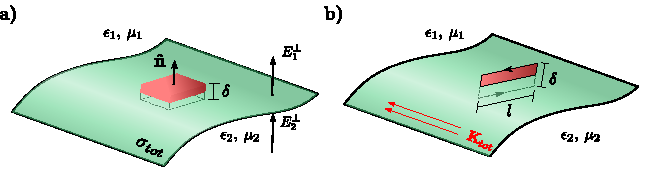
\includegraphics[width=12.5cm]{1-Capitulo-Repaso/0-Diagramas/dibujo.pdf}
	\caption[Condiciones de frontera]{Diagrama de una interfaz (superficie en verde) que separa dos medios homogéneos, lineales e isótropos. El \textit{medio 1} tiene propiedades EM $\epsilon_{1},\,\mu_{1}$, mientras que las del \textit{medio 2} son $\epsilon_{2},\,\mu_{2}$. \textbf{a)} Prisma rectangular con altura $\delta$ y cuyas caras paralelas a la superficie tiene un área $A$. Sobre la superficie que separa a los medios hay una densidad de carga superficial total $\sigma_{tot}$. \textbf{b)} Circuito rectangular con altura $\delta$ y ancho $l$. En la interfaz entre los medios hay una densidad de corriente superficial $\vb{K}_{tot}$.}
	\label{fig:BoundaryConditions} 
\end{figure}
% 

En particular, cuando los medios son lineales, las condiciones de frontera son~\cite{griffiths2013electrodynamics}:
\begin{tcolorbox}[title = Condiciones de frontera para materiales lineales]
	\begin{equation}
	\begin{aligned}
	&\epsilon_{1}E_{1}^{\perp}-\epsilon_{2}E_{2}^{\perp}=\sigma_{tot},&\qquad&\vb{E}_{1}^{\parallel}-\vb{E}_{2}^{\parallel}=\vb{0},\\[2pt]
	&B_{1}^{\perp}-B_{2}^{\perp}=0,&\qquad& \frac{1}{\mu_{1}}\vb{B}^{\parallel}_{1}-\frac{1}{\mu_{2}}\vb{B}^{\parallel}_{2}=\vb{K}_{tot}\times\vu{n}.
	\end{aligned}\label{eq:Condiciones_fronteras_lineal}
	\end{equation}
\end{tcolorbox}
\noindent En las Ecs.~\eqref{eq:Condiciones_fronteras_lineal} es posible notar que, si no hay fuentes externas, tanto componentes paralelas como perpendiculares de los campos EMs son continuas en la frontera entre ambos medios.

\section{Campos eléctromagnéticos armónicos}
Las ecuaciones de Maxwell son cuatro relaciones entre los campos $\vb{E}$, $\vb{B}$, $\vb{D}$ y $\vb{H}$ acopladas, sien embargo es posible separarlas y obtener una ecuación para sólo uno de los campos. Para ello, primero, se observa que, en el vacío y sin fuentes externas, es decir, $\vb{J_{ext}}=\vb{0},\ \rho_{ext}=0$, se cumple que
\begin{eqnarray}
\vb{D}=\epsilon_{0}\vb{E},\qquad\text{y}\qquad\vb{H}=\frac{\vb{B}}{\mu_{0}},~\label{eq:d_h}
\end{eqnarray}
Por otro lado, se calcula el rotacional de la Ec.~\eqref{eq:maxwell4_mat}
\begin{equation}
\curl \curl \vb{H}= - \laplacian \vb{H}= \pdv{\curl\vb{D}}{t},\label{eq:1}
\end{equation}
donde se utilizó la relación~\cite{griffiths2013electrodynamics}
\begin{equation}
\curl\curl\vb{A}= \grad(\div \vb{A}) - \laplacian \vb{A},\label{eq:propiedad}
\end{equation}
y que $\div \vb{H}=0$. Además, se cumple también que $\curl\vb{D}=-\epsilon_{0}\mu_{0}\pdv{\vb{H}}{t}$. \textcolor{red}{Me hiciste la observación de agregar que $\div{\vb{M}}=0$ y $\div{\vb{P}}=0$, pero no creo que sea necesario si desde la Ec~\eqref{eq:d_h} no estoy incluyendo a $\vb{M}$ y $\vb{P}$, o estoy entendiendo algo mal?}Por tanto, sustituyendo en la Ec.~\eqref{eq:1}, se obtiene que~\cite{griffiths2013electrodynamics}
\begin{equation}
\laplacian{\vb{H}}+\epsilon_{0}\mu_{0}\pdv[2]{\vb{H}}{t}=0,\label{eq:ecuacion_de_onda_H}
\end{equation}
A través de un procedimiento análogo se llega a
\begin{equation}
\laplacian{\vb{E}}+\epsilon_{0}\mu_{0}\pdv[2]{\vb{E}}{t}=0, \label{eq:ecuacion_de_onda_E}
\end{equation}
Las Ecs.~\eqref{eq:ecuacion_de_onda_H} y~\eqref{eq:ecuacion_de_onda_E} son la ecuación de onda vectorial para el campo $\vb{H}$ y $\vb{E}$, respectivamente. Cada una de las componentes de los campos $\vb{E}$ y $\vb{H}$ debe satisfacer a la ecuación de onda en su versión escalar. A partir de las Ecs.~\eqref{eq:ecuacion_de_onda_H} y~\eqref{eq:ecuacion_de_onda_E}, la velocidad de la luz se expresa en términos de la permitividad y permeabilidad $c=1/\sqrt{\epsilon_{0}\mu_{0}}$.\\

Una de las soluciones más sencillas a la ecuación de onda escalar está dada por~\cite{griffiths2013electrodynamics}
\begin{equation}
f(\vb{r},t)=Ae^{i\left(\vb{k}\cdot\vb{r}-\omega t\right)},\label{eq:funcion_onda}
\end{equation}
donde $\vb{k}$ es el vector de onda, asociado a la dirección de propagación de la onda, y $\omega$ es la frecuencia angular, da el número de vibraciones en $2\pi$ segundos~\cite{born2005principles}. La amplitud $A$ es una cantidad compleja. La Ec.~\eqref{eq:funcion_onda} también pudo ser escrita en términos de las funciones seno y coseno, sin embargo, es preferible el uso de exponenciales complejas puesto que es más sencillo de manipular para hacer cálculos. Al final, sólo se considera la parte real de la función de onda~\cite{griffiths2013electrodynamics}.\footnote{A partir de la Ec.~\eqref{eq:funcion_onda} se distingue a la onda plana; se obtiene cuando $\vb{k}\cdot\vb{r}$ es constante, por tanto, en cada instante de tiempo $V$ es constante en cada plano definido por $\vb{k}\cdot\vb{r}$~\cite{griffiths2013electrodynamics}.} \\

Debido a la forma de la dependencia temporal en la Ec.~\eqref{eq:funcion_onda} se dice que el campo es armónico en el tiempo. Por ello, los campos EMs armónicos se escriben como~\cite{griffiths2013electrodynamics}
%
\begin{eqnarray}
\vb{E}=\vb{E}_{0}e^{i\left(\vb{k}\cdot\vb{r}-\omega t\right)},&&\vb{H}=\vb{H}_{0}e^{i\left(\vb{k}\cdot\vb{r}-\omega t\right)},\label{eq:Campos_armo}
\end{eqnarray}
para que los campos en la Ec.~\eqref{eq:Campos_armo} puedan ser soluciones a las ecuaciones de Maxwell deben cumplir la relación de dispersión $\omega=kc$. En ausencia de fuentes externas los campos $\vb{E}$ y $\vb{H}$ son ortogonales entre sí y respecto al vector de onda $\vb{k}$ (ver Fig.~\ref{fig:EHFields}). Se relacionan entre sí a través de la siguiente ecuación~\cite{griffiths2013electrodynamics}:
\begin{equation}
\vb{H}=\sqrt{\frac{\epsilon_{0}}{\mu_{0}}}\vb{k}\times\vb{E},
\end{equation}

Debido a la forma de los campos EMs [Ecs.~\eqref{eq:Campos_armo}], las ecuaciones de Maxwell se reescriben como~\cite{bohren1998absorption}
\begin{equation}
\div \epsilon \vb{E}_{c} = 0, 
\label{eq:maxwell1H}
\end{equation}
\begin{equation}
\div \vb{H} = 0, 
\label{eq:maxwell2H}
\end{equation}
\begin{equation}
\curl \vb{E} = i \omega \mu \vb{H}_{c}, 
\label{eq:maxwell3H}
\end{equation}
\begin{equation}
\curl \vb{H} = -i\omega \epsilon \vb{E}_{c}.
\label{eq:maxwell4H}
\end{equation}
Nuevamente, es posible desacoplar las ecuaciones de Maxwell. Para ello calculamos el rotacional de las Ecs. \eqref{eq:maxwell3H} y \eqref{eq:maxwell4H}:
\begin{equation}
\curl (\curl \vb{E})=i\omega \mu \curl \vb{H} = \omega ^{2} \epsilon \mu \vb{E},
\label{eq:curlE}
\end{equation}
\begin{equation}
\curl (\curl \vb{H})=-i\omega \epsilon \curl \vb{E} = \omega ^{2} \epsilon \mu \vb{H}.
\label{eq:curlH}
\end{equation}
Usando la propiedad en la Ec.~\eqref{eq:propiedad}, se reescriben a las Ecs. \eqref{eq:curlE} y \eqref{eq:curlH} como sigue

\begin{tcolorbox}[title = Ecuación vectorial de Helmholtz]\vspace*{-0.3cm}
	\begin{subequations}
		\begin{align}
		\laplacian \vb{E} + \omega^{2} \epsilon \mu \vb{E}&=0, \label{eq:HelmholtzE}\\
		\laplacian \vb{H} + \omega^{2} \epsilon \mu \vb{H}&=0,\label{eq:HelmholtzH}
		\end{align}
	\end{subequations}
\end{tcolorbox}
\noindent en donde $k^{2}=\omega^{2} \epsilon \mu$.

\begin{figure}[ht!]
	\centering
	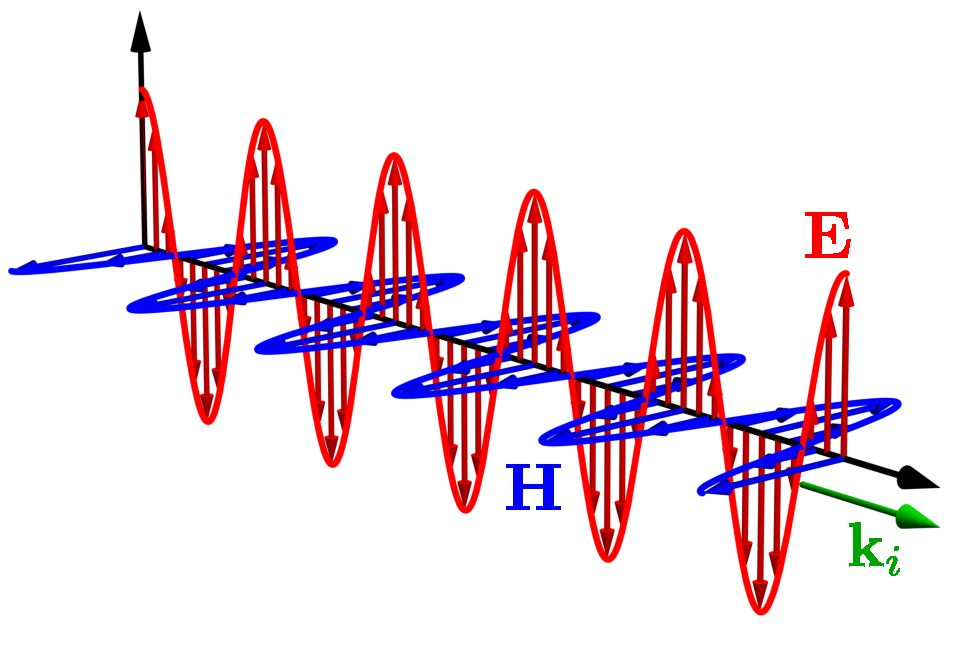
\includegraphics[width=9cm]{1-Capitulo-Repaso/0-Diagramas/campos.pdf}\vspace*{-0.3cm}
	\caption[Campo eléctromagnetico armónico]{Representación de los campos EMs armónicos. En rojo se encuentra el campo eléctrico $\vb{E}$ y en azul el campo $\vb{H}$, para cada uno, las flechas indican la orientación de su oscilación. La flecha verde indica la dirección de propagación de la onda, dada por $\vb{k}_{i}$.}\label{fig:EHFields}
\end{figure}

\section{Vector de Poynting}

El vector de Poynting es una cantidad que indica la energía por unidad de tiempo, por unidad de área, transportada por los campos EMs, de forma general, se define como~\cite{griffiths2013electrodynamics}:
\begin{equation}
\vb{S}=\left(\vb{E} \cross \vb{H}\right).
\label{eq:poynting}
\end{equation}
La energía por unidad de tiempo que cruza una superficie infinitesimal $\dd{\vb{a}}$ es $\vb{S}\cdot\dd{\vb{a}}$, y es llamado flujo de energía~\cite{griffiths2013electrodynamics}.\\

En el caso de la luz, las longitudes de onda, definidas como $\lambda=2\pi/k$, son cortas ($\sim 5\times10^{-7}$ m), y tiene un periodo de oscilación $(2\pi/\omega)$ aproximado de $10^{-15}$ s, por lo que las mediciones macroscópicas involucran muchos ciclos. Por ello no es viable medir directamente al vector de Poynting. Por lo tanto, se utiliza el promedio temporal, denotado con $\expval{...}$~\cite{griffiths2013electrodynamics}. Retomando el caso de campos EMs armónicos, el vector de Poynting luce de la siguiente forma
\begin{equation}
\vb{S} = \Re{\vb{E}} \cross \Re{\vb{H}},
\end{equation}
cuyo promedio temporal es~\cite{born2005principles}
\begin{equation}
\expval{\vb{S}}=\frac{1}{2}\left(\vb{E} \cross \vb{H}^{*}\right),
\label{eq:poynting_promedio}
\end{equation}
en donde el asterisco $^{*}$ indica el complejo conjugado. El cálculo del promedio temporal se realiza sobre un ciclo completo. Ahora es posible calcular la potencia promedio por unidad de área transportada por una onda EM, es decir, la intensidad~\cite{griffiths2013electrodynamics}
\begin{equation}
I=\expval{S}
\end{equation}

Con el vector de Poynting también se determina la magnitud y dirección de la tasa de transferencia de energía electromagnética en cualquier punto del espacio \cite{bohren1998absorption}. Es posible cuantificar la tasa neta con la que la energía EM cruza la frontera de una superficie cerrada $A$ que encierra un volumen $V$~\cite{bohren1998absorption}:
\begin{equation}
W=- \int_{A} \vb{S} \vdot \vu{n} \dd A,
\label{eq:rateElecEnergy}
\end{equation}
donde $\vu{n}$ es el vector unitario normal a la superficie. Es importante notar que se agrega un signo menos en la Ec. \eqref{eq:rateElecEnergy} puesto que se ha elegido el vector normal que apunta hacia afuera del volumen. Entonces, si $\vb{S}$ es tal que apunta en la dirección contraria a $\vu{n}$, W será positiva. Lo cual indica que la energía se absorbe. 

\section{Permitividad eléctrica y permeabilidad magnética}

La permitividad eléctrica y permeabilidad magnética son cantidades esenciales para conocer el comportamiento de los campos EMs en medios materiales. Hasta ahora se han utilizado como escalares, sin embargo, en el caso más general, la permitividad y la permeabilidad son tensores. En el caso de materiales no ferroeléctricos o ferromagnéticos, la presencia de campos eléctricos o magnéticos con intensidad baja induce una polarización o magnetización proporcional a la magnitud del campo aplicado, es decir, la respuesta del medio es lineal. Las componentes cartesianas de $\vb{D}$ y $\vb{H}$ se escriben como~\cite{jackson1999electrodyanmics}
\begin{eqnarray}
D_{i}(\vb{k},\omega)=\sum_{ij}\epsilon_{ij}E_{j}(\vb{k},\omega), \qquad H_{i}(\vb{k},\omega)=\sum_{ij}\mu'_{ij}B_{j}(\vb{k},\omega)\label{eq:def_e_m}
\end{eqnarray}
donde los tensores $\epsilon_{ij}$ y $\mu'_{ij}$ corresponden a la permitividad eléctrica y al inverso de la permeabilidad magnética, respectivamente~\cite{jackson1999electrodynamics}. Además, $\vb{D}(\vb{k},\omega)$ y $\vb{E}(\vb{k},\omega)$ son las transformadas de Fourier de los campos $\vb{D}(\vb{r},t)$ y $\vb{E}(\vb{r},t)$, respectivamente. Si se supone que $\epsilon$ es independiente del vector de onda, al calcular su transformada de Fourier, se llega a que es proporcional a la delta de Dirac $\delta(\vb{r})$. Lo cual indica que $\vb{E}(\vb{r})$ es local, es decir, $\vb{D}(\vb{r})$ depende sólo del campo aplicado en el punto $\vb{r}$. En caso contrario, cuando es no local, la transformada de Fourier es función de $\vb{r}-\vb{r}^{'}$~\cite{yu2010fundamentals}. Los tensores de permeabilidad y permitividad son funciones de la frecuencia y el vector de onda. Dentro del rango visible o radiación electromagnética con longitudes de onda mayores, la no localidad en el espacio es despreciable. Entonces, $\epsilon_{ij}$ y $\mu^{'}_{ij}$ dependen solo de la frecuencia~\cite{jackson1999electrodynamics}.\\


Las Ecs.~\eqref{eq:def_e_m} representan la respuesta lineal del material y dependen de de las estructuras molecular y cristalina dentro de cada material, al igual que de propiedades como la densidad y la temperatura. Los materiales lineales suelen ser isótropos, por tanto, $\epsilon_{ij}$ y $\mu^{'}_{ij}$ son diagonales con todos los elementos iguales, $\vb{D}=\epsilon\vb{E}$ y $\vb{H}=\mu^{'}\vb{B}=\vb{B}/\mu$, que corresponden a las relaciones usadas en las secciones anteriores~\cite{jackson1999electrodynamics}. Puesto que la permitividad y permeabilidad son parte de la relación de dispersión de las ondas EMs planas, es posible anticipar la respuesta general de un material ante una onda EM según la forma de $\epsilon$. La relación de dispersión indica que~\cite{kittel1996introduction}
\begin{equation}
\epsilon(\omega,\vb{k})\epsilon_{0}\mu\omega^{2}=k^{2},
\end{equation}
de donde se concluye que~\cite{kittel1996introduction}
\begin{itemize}
	\item Si $\epsilon$ es un número \textbf{real y positivo}, para $\omega$ real, $k$ es real y una onda EM transversal se propaga en el material.
	\item Si $\epsilon$ es un número \textbf{real y negativo}, para $\omega$ real, $k$ es imaginario y la onda es amortiguada con una longitud característica $1/|k|$.
	\item Si $\epsilon$ es un número \textbf{complejo}, para $\omega$ real, $\vb{k}$ es complejo y las ondas son amortiguadas en el espacio.
\end{itemize}
	
	%Esta parte corresponde a \textbf{Isabel}. El contenido propuesto es
	
	%\begin{itemize}
	% \item Ecuaciones de Maxwell
	% \item Considerar la Ec. de Helmholts
	% \item Hablar sobre los campos EM armónicos
	% \item Vector de Poynting
	% \item Condiciones a la frontera de forma general
	% \item Condiciones a la frontera considerando una esfera
	%\end{itemize}
	
	\chapter{Teoría general de esparcimiento}
	\label{ch:EsparcimientoGral} %-------------------Labels para los capítulos -> ch:LABEL
	
	%!TeX root = ../main.tex

\section{ Matriz de amplitud de esparcimiento}

	\begin{figure}[h!]\centering
	\tdplotsetmaincoords{60}{110}
	\pgfmathsetmacro{\rvec}{1. 3}
	\pgfmathsetmacro{\thetavec}{30}
	\pgfmathsetmacro{\varphivec}{60}
\begin{tikzpicture}[scale=3.5,tdplot_main_coords]
%draw the NP
%	\draw[tdplot_screen_coords,ball color=yellow, opacity = 1] (0,0,0) circle (.05);
%	\draw[tdplot_screen_coords, color=yellow, opacity = 1] (0,0,0) circle (.05);
\pgfmathsetseed{3}
\draw[tdplot_screen_coords, ball color=yellow, opacity = 1,scale =.1]
	 plot [smooth cycle, samples=8,domain={1:8}]
     (\x*360/8+5*rnd:0.5cm+1cm*rnd) node at (0,0) {};
\pgfmathsetseed{3}    
\draw[tdplot_screen_coords, color=yellow, opacity = 1,scale =.1]
	 plot [smooth cycle, samples=8,domain={1:8}]
     (\x*360/8+5*rnd:0.5cm+1cm*rnd) node at (0,0) {};
%set up some coordinates 
	\coordinate (O) at (0,0,0);

%determine a coordinate (P) using (r,\theta,\varphi) coordinates.   This command
%also determines (Pxy), (Pxz), and (Pyz): the xy-, xz-, and yz-projections
%of the point (P). 
%syntax: \tdplotsetcoord{Coordinate name without parentheses}{r}{\theta}{\varphi}
	\tdplotsetcoord{P}{\rvec}{\thetavec}{\varphivec}

%draw figure contents
%--------------------
%draw the main coordinate system axes
	\draw[thick,- latex] (0,0,0) -- (1. 5,0,0) node[anchor=north east]{$x$};
	\draw[thick,- latex] (0,0,0) -- (0,1. 5,0) node[anchor=north west]{$y$};
	\draw[thick,- latex] (0,0,0) -- (0,0,1. 5) node[anchor=south]{$z$};

%draw the main cartesian vector system 
	\draw[thick,- latex, blue] (0,0,0) -- (1,0,0) node[anchor= south east]{$\vu{e}_x$};
	\draw[thick,- latex, blue] (0,0,0) -- (0,1,0) node[anchor=north west]{$\vu{e}_y$};
	\draw[thick,- latex, blue] (0,0,0) -- (0,0,1) node[anchor= east]{$\vu{e}_z$};

%draw a vector from origin to point (P) 
	\draw[thick,color=green, - latex] (O) -- (P);
	\node at (1,. 5,1. 1) {\color{green} $\vb{r}$};

%draw projection on xy plane, and a connecting line
	\draw[dashed, color=green] (O) -- (Pxy);
	\draw[dashed, color=green] (P) -- (Pxy);
	\fill[green, opacity = .3] (O) --(Pxy)-- (P)--(O);
	\draw[- latex, tdplot_screen_coords,green](.42,.2)--(.8,.2);
	\node[tdplot_screen_coords] at (1.35,.2) {\color{green}\small Plano de esparcimiento};


%draw the angle \varphi, and label it
	%syntax: \tdplotdrawarc[coordinate frame, draw options]{center point}{r}{angle}{label options}{label}
	\tdplotdrawarc[- latex]{(O)}{0. 5}{0}{\varphivec}{anchor=south}{$\varphi$}


%set the rotated coordinate system so the x'-y' plane lies within the
	%"theta plane" of the main coordinate system
	%syntax: \tdplotsetthetaplanecoords{\varphi}
	\tdplotsetthetaplanecoords{\varphivec}

%draw theta arc and label, using rotated coordinate system
	\tdplotdrawarc[tdplot_rotated_coords, - latex]{(0,0,0)}{0. 45}{0}{\thetavec}{anchor=north}{$\theta$}

%draw some dashed arcs, demonstrating direct arc drawing
	\draw[dashed,tdplot_rotated_coords] (\rvec,0,0) arc (0:90:\rvec);
	\draw[dashed] (\rvec,0,0) arc (0:90:\rvec);

%set the rotated coordinate definition within display using a translation
%coordinate and Euler angles in the "z(\alpha)y(\beta)z(\gamma)" euler rotation convention
%syntax: \tdplotsetrotatedcoords{\alpha}{\beta}{\gamma}
	\tdplotsetrotatedcoords{\varphivec}{\thetavec}{0}

%translate the rotated coordinate system
%syntax: \tdplotsetrotatedcoordsorigin{point}
	\tdplotsetrotatedcoordsorigin{(P)}

%use the tdplot_rotated_coords style to work in the rotated, translated coordinate frame
	\draw[thick,tdplot_rotated_coords,- latex, purple] (0,0,0) -- (. 3,0,0) node[anchor=north west]{{\color{orange}$\vu{e}_\theta,$}$\vu{e}_{\parallel}^s$};
	\draw[thick,tdplot_rotated_coords,- latex,orange] (0,0,0) -- (0,. 3,0) node[anchor=west]{$\vu{e}_\varphi$};
	\draw[thick,tdplot_rotated_coords,- latex,purple] (0,0,0) -- (0,-. 3,0) node[anchor= north west]{$\vu{e}_{\perp}^s$};
	\draw[thick,tdplot_rotated_coords,- latex, orange] (0,0,0) -- (0,0,. 3) node[anchor=south]{$\vu{e}_r$ };



%set the rotated coordinate definition within display using a translation
%coordinate and Euler angles in the "z(\alpha)y(\beta)z(\gamma)" euler rotation convention
%syntax: \tdplotsetrotatedcoords{\alpha}{\beta}{\gamma}
	\tdplotsetrotatedcoords{\varphivec}{0}{0}

%translate the rotated coordinate system
%syntax: \tdplotsetrotatedcoordsorigin{point}
	\tdplotsetrotatedcoordsorigin{(Pxy)}

	\draw[thick,tdplot_rotated_coords,- latex, purple] (0,0,0) -- (. 3,0,0) node[anchor= west]{$\vu{e}_{\parallel}^i$};
	\draw[thick,tdplot_rotated_coords,- latex, blue] (0,0,0) -- (0,0,. 3) node[anchor= west]{$\vu{e}_z$};	
	\draw[thick,tdplot_rotated_coords,- latex, purple] (0,0,0) -- (0,-. 3,0) node[anchor= north west]{$\vu{e}_{\perp}^i$};



% Plane Wave
	\foreach \i in {-7,...,-2}{
		\draw[thick,tdplot_screen_coords,red, - latex] (\i/10,0,0)--(\i/10,1,0);}
	\node[tdplot_screen_coords] at (-4.5/10,1.1,0){\color{red}$\vb{k}_i$};
	\node[tdplot_screen_coords] at (-4.5/10,-.1,0){\small \color{red}Haz incidente};
\end{tikzpicture}
%
\caption{Diagrama del plano de esparcimiento (en verde) definido por el vector $\vb{r}$, posición donde se evalúan los campos EMs, y el vector $\vu{e}_z$, cuando una onda plana monocromática propagándose en dirección $z$ (en rojo) ilumina a una partícula arbitraria.  La base cartesiana para vectores se muestra en azul, mientras que la base esférica se muestra en negro.  Las direcciones paralelas $\parallel$ y perpendiculares $\perp$ al plano de incidencia  para el campo eléctrico incidente, denotado por el subíndice $i$ y el esparcido, denotado por el subíndice $s$, se muestran en morado; el haz incidente se muestra en rojo.}\label{fig:PlanoEsparcimiento}
	\end{figure}	

Para  el estudio del esparcimiento por una partícula arbitraria inmersa en un medio con índice de refracción $n_m$, denominado  matriz, se considera que la partícula es iluminada por una onda plana monocromática con una longitud de onda $\lambda$, cuya dirección de propagación define la dirección $z$, es decir,
	\begin{align}
	\vb{E}^i = (E_x^i \vu{e}_x + E_y^i \vu{e}_y)e^{i(k z - \omega t)},
	\label{eq:Exyi}
	\end{align}
donde $k = 2\pi n_m /\lambda$ es el número de onda. En la Fig.  \ref{fig:PlanoEsparcimiento} se muestra  una partícula localizada en el origen,  iluminada por una onda plana monocromática [Ec. \eqref{eq:Exyi}] que se propaga en la dirección $z$; sobre la partícula se posiciona el origen del sistema coordenado cartesiano ($x,y,z$). Adicionalmente, en la Fig. \ref{fig:PlanoEsparcimiento} se muestran en las bases de vectores ortonormales retangulares \{$\vu{e}_x,\vu{e}_y,\vu{e}_z$\} en azul, y los polares \{$\vu{e}_r,\vu{e}_\theta,\vu{e}_\varphi$\} en naranja. De forma análoga al plano de incidencia\footnote{En el problema de un haz de luz incidente a una superficie plana, el plano de incidencia se define por el vector normal a
la superficie y la dirección de propagación del haz.}, se construye el plano de esparcimiento (en verde en la Fig. \ref{fig:PlanoEsparcimiento}), con el vector de la dirección de esparcimiento $\vu{e}_r$ y la dirección del haz incidente $\vu{e}_z$, que define las componentes ortogonales $\perp$ y paralelas $\parallel$ de los campos EMs, así como su polarización. \index{Plano!de esparcimiento} \index{Polarización!respecto al plano de esparcimiento} Los vectores unitarios perpendicular y paralelo al plano de esparcimiento de la onda plana incidente, $\vu{e}_{\perp}^i$  y $\vu{e}_{\parallel}^i$, respectivamente se muestran en morado en la Fig. \ref{fig:PlanoEsparcimiento} y están dados por%
\begin{subequations} \index{Polarización!respecto al plano de esparcimiento!paralela ($\parallel$)}\index{Polarización!respecto al plano de esparcimiento!perpendicular ($\perp$)}
%
	\begin{align}
	\vu{e}_{\perp}^i &=- \vu{e}_\varphi  = \sin\varphi\,\vu{e}_x - \cos\varphi\,\vu{e}_y, \\
	\vu{e}_{\parallel}^i &= \cos\varphi\,\vu{e}_x + \sin\varphi\,\vu{e}_y,\\
	\vu{e}_z &= \cos\varphi\vu{e}_x+\sin\varphi\vu{e}_y.
		\end{align}
	\label{eqs:vecInc}\end{subequations}
%
Asimismo, los vectores unitarios de los campos electromagnéticos (EMs) esparcidos por la partícula en la dirección perpendicular y paralela al campo de esparcimiento, $\vu{e}^s_\perp$ y $\vu{e}^s_\parallel$, son
%	
	\begin{subequations}\begin{align}
	\vu{e}_{\perp}^s &= - \vu{e}_\varphi = \vu{e}_{\perp}^i,\\
	\vu{e}_{\parallel}^s &= \vu{e}_\theta,\\
	\vu{e}_r &= \vu{e}_\perp^s\times\vu{e}_\parallel^s.
	\end{align}	\label{eqs:vecScat}\end{subequations}
%
Al despejar $\vu{e}_x$ y $\vu{e}_y$  de las Ecs. \eqref{eqs:vecInc} y reescribirlos en la base de los vectores unitarios en la dirección perpendicular y normal al plano de esparcimiento, como $\vu{e}_x = \sin\varphi\,\vu{e}_{\perp}^i + \cos\varphi\,\vu{e}_{\parallel}^i$ y $\vu{e}_y = - \cos\varphi \,\vu{e}_{\perp}^i + \sin\varphi\,\vu{e}_{\parallel}^i$, se obtiene que el campo eléctrico incidente $\vb{E}^i$ [Ec. \eqref{eq:Exyi}] se puede escribir como
%
\begin{align}
\vb{E}^i &= [(\cos\varphi E_{x}^i + \sin\varphi E_{y}^i)\vu{e}_{\perp}^i +
			 (\sin\varphi E_{x}^i - \cos\varphi E_{y}^i)\vu{e}_{\parallel}^i]
			 e^{ikz}
			 \label{eq:EIncidenteFull} \\
			 &= E_{\perp}^i  \vu{e}_{\perp}^i + E_{\parallel}^i\vu{e}_{\parallel}^i,
		\label{eq:EIncidente}
\end{align}
%
en donde se omite el término de la fase temporal $e^{-i\omega t}$ y la fase espacial $e^{ikz}$ se incluye en los coficientes $E_\perp^i$ y $E_\parallel^i$. 

En el problema de esparcimiento por una partícula, la cantidad que se mide experimentalmente es la
intensidad de la luz, que es una cantidad proporcional al vector de Poynting [Ec. \eqref{eq:poynting}] en la región de campo lejano, es decir que las expresiones de los campos EMs se calculan considerando $kr\gg 1$. Para calcular a los campos EMs producidos por una fuente oscilante en la región de campo lejano, consideremos el potencial vectorial $\vb{A}(\vb{r},t)$ con la norma de Lorentz \footnote{Ver sección 9.1 de \cite{jackson1999electrodynamics}.} dado por la expresión
%
\begin{align}
\vb{A}(\vb{r},t) = \frac{\mu_0}{4\pi}\int_{V'}\vb{J}(\vb{r}')\frac{e^{ik\norm{\vb{r}-\vb{r}'}}}{\norm{\vb{r}-\vb{r}'}} \dd^3r'e^{-i\omega t},
 \label{eq:AFuenteOscilante}
\end{align}
%
y a su vez, los campos $\vb{H}$ y $\vb{E}$, que asumimos armónicos en el tiempo, están dados por
%
\begin{align}
\vb{H} &= \frac{1}{\mu_0}\nabla\times\vb{A},
\label{eq:H=curlA}\\
\vb{E} &= \frac{i}{k}\sqrt{\frac{\mu_0}{\varepsilon_0}}\nabla\times\vb{H}.
\label{eq:E=curlcurlA}
\end{align}
%
Dado que nos interesa la región del espacio tal que $kr\gg 1$, entonces $\norm{\vb{r}-\vb{r}'}\approx r-\vu{e}_r\cdot\vb{r}'\approx r$. Sustituyendo este resultado en la Ec. \eqref{eq:AFuenteOscilante}, obtenemos que
%
\begin{align}
\vb{A}(\vb{r},t) &\approx \frac{\mu_0}{4\pi}\frac{e^{ikr}}{r}\int_{V'}\vb{J}(\vb{r}')\dd^3r'\\
		&=  \frac{\mu_0}{4\pi}\frac{e^{ikr}}{r}\qty[
			\int_{V'}-\vb{r}'\bigg(\nabla'\cdot\vb{J}(\vb{r}')\bigg)\dd^3r'	+\int_{ V'}\nabla'\cdot\bigg(\vb{J}(\vb{r}')\vb{r}'\bigg)\dd^2r'],\\
		&= \frac{\mu_0}{4\pi}\frac{e^{ikr}}{r}\qty[
			\int_{V'}-\vb{r}'\bigg(\nabla'\cdot\vb{J}(\vb{r}')\bigg)\dd^3r'	+\int_{\partial V'}\bigg(\vb{J}(\vb{r}')\vb{r}'\bigg)\cdot\vu{n}\dd^2r'],
\label{eq:AintEspFrontera}
\end{align}
%
donde realizamos una integración por partes y empleamos el teorema de la divergencia. Si consideramos nuestro volumen de integración como todo el espacio, y dado que nuestra fuentes de un tamaño finito, la integral de superficie en la Ec.\eqref{eq:AintEspFrontera} es cero. Finalmente,  sustituyendo con la ecuación de continuidad ($\nabla\cdot\vb{J} = i\omega\rho$, con $\rho$ la densidad de carga) podemos escribir el potencial vectorial como 
%
\begin{align}
\vb{A}(\vb{r},t)  \approx -\frac{i\mu_0\omega}{4\pi}\frac{e^{ikr}}{r}\vb{p},\qquad
\text{con}\qquad \vb{p} = \int_{V'}\vb{r}'\rho(\vb{r}')\dd^3r',
\label{eq:Aoscilante}
\end{align}
%
en donde $\vb{p}$ es el momento dipolar.

Al emplear la Ec. \eqref{eq:Aoscilante} para calcular el campo magnético con la Ec. \eqref{eq:H=curlA} (\ref{ex:Hoscilante}) obtenemos que
%
\begin{align}
\vb{H} = \frac{ck^2}{4\pi}\frac{e^{ikr}}{r}\qty(1-\frac{1}{ikr})\vu{e}_r\times\vb{p}.
\label{eq:Hoscilante}
\end{align}
%
El campo eléctrico se calcula empleando la Ec. \eqref{eq:E=curlcurlA} con el resultado de la Ec. \eqref{eq:Hoscilante}; tras una manipulación algebráica (\ref{ex:Eoscilante}) podemos reescribir al campo eléctrico en una contribución de campo lejano (que decae como $r^{-1}$) y de campo cercano (que decae como $r^{-n}$ con $n\geq 2$) como \cite{jackson1999electrodynamics} como
%
\begin{align}
\vb{E} = \frac{e^{ikr}}{4\pi\varepsilon_0}\qty[
\mathrlap{\underbrace{\phantom{\frac{k^2}{r}\qty(\vu{e}_r\times\vb{p})\times\vu{e}_r }}_{\text{Campo lejano}}}
\frac{k^2}{r}\qty(\vu{e}_r\times\vb{p})\times\vu{e}_r
+
\mathrlap{\underbrace{\phantom{[3\vu{e}_r\qty(\vu{e}_r\cdot\vb{p})-\vb{p}]\qty(\frac{1}{r^3}-\frac{ik}{r^2})}}_{\text{Campo cercano}}}
[3\vu{e}_r\qty(\vu{e}_r\cdot\vb{p})-\vb{p}]\qty(\frac{1}{r^3}-\frac{ik}{r^2})
].
\label{eq:Eoscilante}
\end{align}
%

Al considerar para el campo eléctrico esparcido  $\vb{E}^s$ únicamente los términos que corresponden al campo lejano de la Ec. \eqref{eq:Eoscilante}, el campo esparcido cumple con que $kr\ll 1$, además de ser transversal a la dirección de propagación. Por lo tanto, el campo esparcido puede escribirse como \cite{bohren1998absorption}\index{Electromagnéticos!campos!lejano} 
%
	\begin{align}
	\vb{E}^{sca} \propto \frac{e^{ikr}}{-ikr}\vb{E}_0^{sca}
			=  \frac{e^{ikr}}{-ikr}
			\qty( E_{\perp}^s  \vu{e}_{\perp}^s + E_{\parallel}^s \vu{e}_{\parallel}^s), \label{eq:ELejano}
	\end{align}
%	
en donde  $\vb{E_0}^{sca}$ es la amplitud del campo esparcido,  $ E_{\perp}^s$ y  $ E_{\parallel}^s$ sus componentes en la base de los vectores paralelo y perpendicular al plano de esparcimiento [Ec. \eqref{eqs:vecScat}]. Asimismo, es posible relacionar al campo eléctrico esparcido $\vb{E}^{sca}$ por una partícula localizada en el centro de coordenadas  [Ec. \eqref{eq:ELejano}] con el  campo eléctrico incidente $\vb{E}^i$ [Ec. \eqref{eq:EIncidente}],  mediante el operador de esparcimiento de campo lejano  $\mathbb{F}(\vu{k}^i,\vu{k}^s)$ \index{Electromagnéticos!campos!operador de campo lejano} \cite{tsang2000scattering}
%
	\begin{align}
	\vb{E}^{sca} = \frac{e^{i\vb{k}^{s}\cdot\vb{r}}}{r}\mathbb{F}(\vu{k}^i,\vu{k}^{s})\vb{E}^i,
	\label{eq:FarFieldDyadic}
	\end{align}
%	
donde $\mathbb{F}$ depende de la dirección de la onda plana incidente $\vu{k}^i$ y de la dirección del campo eléctrico esparcido $\vu{k}^{s}$. El operador $\mathbb{F}$ denota que, en general, el campo esparcido puede tener una polarización distinta a la de la onda plana incidente y también puede tener una fase distinta. Al considerar la forma asintótica del campo eléctrico esparcido [Ec. \eqref{eq:ELejano}] y su relación con el campo eléctrico incidente [Ec. \eqref{eq:FarFieldDyadic}], se pueden relacionar las componentes perpendiculares del campo esparcido y el campo incidente de una onda plana en la base de los vectores perpendiculares y paralelos al plano de incidencia mediante la matriz de amplitud esparcimiento $\mathbb{S}$ \index{Esparcimiento!matriz de} \cite{bohren1998absorption}
%
	\begin{tcolorbox}[title = Matriz de amplitud de esparcimiento $\mathbb{S}$, ams align ]
\mqty(E_{\parallel}^s\\E_{\perp}^s) = 
		\frac{e^{ik(r-z)}}{-ikr} \mqty(S_2&S_3\\S_4&S_1)
	\mqty(E_{\parallel}^i\\E_{\perp}^i),\label{eq:MEsparcimientoGral}		
	\end{tcolorbox} 
%
\noindent
en donde los elementos de matriz $S_j = S_j(\theta,\varphi)$ con $j=1,2,3$ y $4$, son funciones complejas que dependen de la geometría de la partícula iluminada por la onda plana.
	%!TeX root = ../main.tex
\section{Esparcimiento, extinción y absorción}

En la sección anterior, se estudió cómo se relaciona el campo eléctrico que incide en una partícula arbitraria con el campo eléctrico esparcido por esta, dando como resultado la relación de la Ec. \eqref{eq:MEsparcimientoGral}. En esta sección, se estudia el balance de energía al presentarse el fenómeno de esparcimiento.

Supóngase un haz de luz cruza por un medio donde se encuentran partículas arbitrarias (ver Fig. \ref{fig:EnergiaDetector}) y que la energía medida por un detector colocado detrás de las partículas  es $U$. En el caso donde no hubiera partículas, la energía que mediría el detector sería $U_0$ , con $U_0 > U$.  La diferencia de energía $U_0-U$ entre ambos casos es atribuida tanto a la absorción de las partículas (conversión de la energía EM en otras formas de energía, como calor), como al esparcimiento de la luz en direcciones distintas a la posición del detector. Al efecto en conjunto de la absorción y del esparcimiento se denomina extinción.

	\begin{figure}[h!]\centering
%	\tdplotsetmaincoords{60}{110}
%	\pgfmathsetmacro{\rvec}{1. 3}
%	\pgfmathsetmacro{\thetavec}{30}
%	\pgfmathsetmacro{\varphivec}{60}
\begin{tikzpicture}[scale=3.5]
\def\d{.75}

%------- Scatterers cloud
\foreach \i in {0,20,40,60,...,360}{
\pgfmathsetseed{\i}
\draw[ball color=yellow, opacity = 1,scale =.03,rotate = rnd, shift={({10*rnd*cos(\i)},{10*rnd*sin(\i)})}]
	 plot [smooth cycle, samples=8,domain={1:8}]
     (\x*360/8+5*rnd:0.5cm+1cm*rnd) node at (0,0) {};
}
%------ Incident wave
	\foreach \i in {-3,...,3}{
		\draw[thick,red, - latex] (-1.5,\i/20)--(-.5,\i/20);}
	\node at (-1.2,5/20){\small \color{red}Haz incidente};	
	\node at (-.75, 5/20) {\small \color{red}$\vb{k}^i$};
%------ Transmitted wave	
	\foreach \i in {-1,...,1}{
\draw[thick,red, - latex] (.5,\i/20)--(1.25,\i/20);}
\node at (.85,3/20){\small \color{red}Haz transmitido};	

%------- Detector
\node at ( 1.5, -6/20){\small Detector};
\begin{scope}[scale  = .25, shift = {(3.5,-2.3)}, rotate = 90, shift = {(-.25,-5)}]
\shade[left color=gray!50!white,right color=gray] (1.7,3)
    -- ++(1.6,0) -- ++(-0.3,-1) -- ++(-1,0) -- cycle;% column
  \shade[left color=gray!50!white,right color=gray] (2.1,2)
    -- ++(0.8,0) -- ++(0,-0.2) -- ++(-0.8,0) -- cycle;% column bottom
  \draw[gray!80!black] (1.7,3) -- ++(1.6,0) -- ++(-0.3,-1)
    -- ++(-1,0) -- cycle;%column
  \draw[gray!80!black] (2.1,2) -- ++(0,-0.2) -- ++(0.8,0)
    -- ++(0,0.2);%column bottom
\end{scope}	

%------- Campo esparcido
\node at ( .5, -8/20){\small Haz esparcido};
\begin{scope}[opacity=1, transparency group, scale = .15]
\foreach \s in {-1,1}{
	\draw[- latex, red](0,\s*\d)++(25:\s*1.75)--(35+rand*5:\s*3.5);
	\draw[- latex, red](0,\s*\d)++(35:\s*1.3)--(55+rand*5:\s*2.75);
	\draw[- latex, red](0,\s*\d)++(165:\s*2)--(155+rand*5:\s*3);
	\draw[- latex, red](0,\s*\d)++(120:\s*1.75)--(110+rand*5:\s*3.5);
	\draw[- latex, red](0,\s*\d)++(60:\s*1.5)--(60+rand*5:\s*4);}
\end{scope}

\end{tikzpicture}
%
\caption{Diagrama de la extinción de luz por una nube de partículas esparcidoras. La energía que mide el detector en la ausencia de partículas es $U_0$ sin embargo, al interactuar la luz con las partículas, la lectura de energía es $U$. La energía $U-U_0$  corresponde a la energía que no llega al detector asociada tanto al esparcimiento de luz, como a la absorbida por las partículas; al conjunto de estos fenómenos se le denomina extinción.}\label{fig:EnergiaDetector}
	\end{figure}	
	
Ahora, considérese el caso de una sola partícula (de tamaño  forma arbitraria) inmersa en un medio dispersor e iluminada por una onda plana; debido a la onda plana, la partícula esparce luz.  Para cuantificar la energía esparcida por la partícula, defínase una esfera $A$ de radio $r$ que contenga a la partícula. La energía total  por unidad de tiempo que cruza la superfice de $A$ se calcula como
%
\begin{align}
W_{abs} = -\int_A \ev{\vb{S}}_t\cdot \vu{e}_r \dd{a},
\label{eq:Wa}
\end{align}
%
donde $\ev{\cdot}_t$ denota el promedio temporal, y donde el vector de Poyntig $\vb{S}$ puede descomponerse en tres contribuciones:
%
\begin{align}
\ev{\vb{S}}_t &= \frac12 \Re[\vb{E}\times\vb{H}^*] = \ev{\vb{S}^i}_t + \ev{\vb{S}^{sca}}_t + \ev{\vb{S}^{ext}}_t,
\label{eq:PoyntingContribuciones}\\
\ev{\vb{S}^i}_t &= \frac12 \Re[\vb{E}^i\times\vb{H}^{*i}], \\
\ev{ \vb{S}^{sca}}_t &= \frac12 \Re[\vb{E}^{sca}\times\vb{H}^{sca*}] ,\\
\ev{\vb{S}^{ext}}_t &= \frac12 \Re[\vb{E}^i\times\vb{H}^{sca*} + \vb{E}^{sca} \times\vb{H}^{i*}],
\label{eq:Sext}
\end{align}
%
siendo $i$ y $sca$ los subíndices que denotan a los campos EMs incidentes y esparcidos (\textit{scattering} en inglés), respectivamente, mientras que $ext$ corresponde al campo EMs resultado de la interferencia entre la onda incidente y los campos esparcidos; a este término lo asociaremos a la extinción.

Según la Ec \eqref{eq:Wa}, si $W_{abs}>0$ entonces la energía es absorbida dentro de la esfera, y si $W_{abs}<0$ entonces energía es generada en la partícula, aunque a lo largo de este texto se excluye este caso. Al descomponer a $W_{abs}$ en las mismas contribuciones que al  vector de Poynting en la Ec. \eqref{eq:PoyntingContribuciones}, obtenemos que
%
\begin{align}
W_{abs} &= W_i - W_{sca} + W_{ext},
\end{align}
%
con
%
\begin{align}
W_{i} &= -\int_A\ev{\vb{S}^i}_t\cdot \vu{e}_r \dd{a} = 0,\\
W_{sca} &= \int_A\ev{\vb{S}^{sca}}_t\cdot \vu{e}_r \dd{a},\label{eq:Wsca}\\
W_{ext} &= -\int_A\ev{\vb{S}^{ext}}_t\cdot \vu{e}_r \dd{a},
\end{align}

donde $W^i=0$ dado que la partícula se encuentra en un medio no disipativo. Es decir, que la energía extinta por unidad de tiempo es
%
\begin{align}
W_{ext} = W_{abs} + W_s,
\end{align}
%
como se describió al inicio de esta sección.	

Como caso particular, supóngase que la onda plana incidente está polarizada en la dirección $x$, es decir que $\vb{E}^i = E_0\vu{e}_x$, con $E_0$	 la amplitud del campo eléctrico incidente. Empleando la  expresión para el campo eléctrico esparcido $\vb{E}^{sca}$ como función del campo incidente [Ec. \eqref{eq:MEsparcimientoGral}] y empleando la Ec. \eqref{eq:EIncidenteFull}, así como la ley de Faraday-Lenz, los campos EMs esparcidos se escriben como
%
\begin{align}
\vb{E}^{sca}(\vb{r}) &= \frac{e^{ik(r-z)}}{-ikr}E_0\vb{X}(\theta,\varphi),
\label{eq:EscaX}\\
\vb{H}^{sca}(\vb{r}) &= \frac{e^{ik(r-z)}}{kr\omega\mu}E_0\vu{e}_r\times\vb{X}(\theta,\varphi),
\label{eq:HscaX}
\end{align}
%
con $\vb{X}\cdot\vu{e}_r = 0$ dada por
%
\begin{align}
\vb{X}(\theta,\varphi) = (S_2\cos\varphi + S_3\sin\varphi)\vu{e}_{\parallel}^{s} + (S_4\cos\varphi + S_1\sin\varphi)\vu{e}_{\perp}^{s},
\end{align}
%
donde $S_j = S_j(\theta,\varphi)$.

Para calcular la energía por unidad de tiempo $W_{ext}$ asociada a la extinción que cruza a una superficie esférica $A$ de radio $r$, se emplean las Ecs. \eqref{eq:Sext}, \eqref{eq:EscaX} y \eqref{eq:HscaX}  (\ref{ex:Wext}), dando como resultado que
%	
\begin{align}
W_{ext} &= -\int_{A} \ev{\vb{S}^{ext}}_t\cdot\vu{e}_r\dd{a}\notag\\
 &= \frac{kE_0^2}{2\mu\omega}\Re\bigg\{
\frac{e^{-ikr}}{-ikr}
	\int_A e^{ikz} (\vu{e}_x\cdot\vb{X}^*)\dd{a}\notag\\
&\qquad\qquad+\frac{e^{ikr}}{ikr}
	\int_A e^{-ikz}(\vb{X}\cdot\vu{e}_x)\cos\theta\dd{a}\notag\\
&\qquad\qquad-\frac{e^{ikr}}{ikr}
	\int_A e^{-ikz}(\vb{X}\cdot\vu{e}_z)\sin\theta\cos\varphi\dd{a}
	\bigg\},
	\label{eq:WextX}
\end{align}
donde $ikz = ikr\cos\theta$ y $\dd{a} =r^2 \sin\dd{\theta}\dd{\varphi}$. Para resolver las integrales de la Ec. \eqref{eq:WextX}, empleemos dos veces la integración por partes el siguiente caso general con $\mu = \cos\theta$ 
%
\begin{align}
\int_{-1}^{1} e^{\pm ikr\mu}f(\mu)\dd{\mu} = \pm
f(\mu)\frac{e^{\pm ikr\mu}}{ikr}\eval_{-1}^1 -
\frac{\mp 1}{(kr)^2}\qty(
\dv{f(\mu)}{\mu}e^{\pm ikr\mu}\eval_{-1}^1 -\int_{-1}^1\dv[2]{f(\mu)}{\mu}e^{\pm ikr\mu}\dd{\mu}
).
\label{eq:eikmu}
\end{align}
%
Dado que consideramos una región del espacio tal que $kr\gg 1$, la expresión de la Ec. \eqref{eq:eikmu} se aproxima a
%
\begin{align}
\int_{-1}^{1} e^{\pm ikr\mu}f(\mu)\dd{\mu} \approx \frac{\pm 1}{ikr}\qty(f(1) e^{\pm ikr} - f(-1)e^{\mp ikr}).
\label{eq:approxInt}
\end{align}
%
Escogiendo $f_1(\mu) = 1, f_2(\mu) = \mu$ y $f_3(\mu) = \sqrt{1-\mu^2}$ para los integrandos de la Ec. \eqref{eq:WextX} y empleando la aproximación de la Ec. \eqref{eq:approxInt}, vemos que la integral con el término $f_3$ se anula, por lo que la única contribución es\footnote{Al escribir $\vb{X}$ en la base cartesiana canónica, esta cantidad no depende de $\varphi$, por lo que la integral en esta variable es $2\pi$.}
%
\begin{align}
W_{ext} &=  \frac{2\pi kE_0^2}{2\mu\omega k^2}\Re\bigg\{
e^{-ikr}\qty[
 e^{ikr} (\vu{e}_x\cdot\vb{X}^*) \eval_{\theta=0} - e^{-ikr} (\vu{e}_x\cdot\vb{X}^*) \eval_{\theta=\pi}
 ] \notag \\
&\qquad\qquad\qquad+e^{ikr}\qty[
 e^{-ikr}(\vb{X}\cdot\vu{e}_x)\eval_{\theta=0} + e^{ikr}(\vb{X}\cdot\vu{e}_x)\eval_{\theta = \pi}
	 ]
	\bigg\},\\
	&=  \frac{2\pi kE_0^2}{2\mu\omega k^2}\Re\bigg\{
\qty[
(\vb{X}\cdot\vu{e}_x)\eval_{\theta=0} +
 (\vu{e}_x\cdot\vb{X}^*) \eval_{\theta=0} 
 ]\notag \\
&\qquad\qquad\qquad+\qty[e^{2ikr}(\vb{X}\cdot\vu{e}_x)\eval_{\theta = \pi} - e^{-2ikr} (\vu{e}_x\cdot\vb{X}^*) \eval_{\theta=\pi}
	 ]
	\bigg\}.
\end{align}
%
Los términos entre paréntesis pueden reescribirse como $2\Re\{\vb{X}\cdot\vu{e}_x\}$, evaluado en $\theta = 0$, y $2i\Im\{e^{2ikr}(\vb{X}\cdot\vu{e}_x)\}$	, evaluado en $\theta = \pi$, por lo que al calcular la parte real, concluimos que la energía  asociada a la extinción  por unidad de tiempo que cruza una superficie esférica es
%
\begin{align}
W_{ext} = \qty(\frac{kE_0^2}{2\mu\omega})\frac{4\pi}{k^2} \Re\qty[(\vb{X}\cdot\vu{e}_x)\eval_{\theta = 0 }] = I_i \frac{4\pi}{k^2}\Re\qty[(\vb{X}\cdot\vu{e}_x)\eval_{\theta = 0 }],
\label{eq:WextXFull}
\end{align}
% 
donde $I_i$ es la irradiancia (energía por unidad de tiempo por unidad de área) de la onda plana incidente. El término que multiplica a $I_i$ en la Ec. \eqref{eq:WextXFull} tiene unidades de área y se le conoce como la sección transversal de extinción, dada por la expresión
%
\begin{align}
C_{ext,x} = \frac{4\pi}{k^2}\Re\qty[(\vb{X}\cdot\vu{e}_x)\eval_{\theta = 0 }],
\label{eq:Cextx}
\end{align}
%
con el subíndice $x$ denotando explícitamente la polarización de la onda plana incidente. Se forma semejante, se definen las secciones transversales de absorción $C_{abs} = W_{abs}/I_i$ y de esparcimiento $C_s = W_s/I_i$, que se relacionan por medio de la Ec.  \eqref{eq:Wa} cumpliendo que
%
\begin{align}
C_{ext} = C_{abs} + C_{sca}.
\label{eq:C-All}
\end{align}
%

Para obtener una expresión de $C_{sca}$, calculemos  $W_{sca}$ [Ec. \eqref{eq:Wsca}] con los campos EMs esparcidos [Ecs. \eqref{eq:EscaX} y \eqref{eq:HscaX}] considerando, nuevamente, una onda plana incidente polarizada en la dirección $x$. Al dividir $W_{sca}$ por la irradiancia de una onpla plana, obtenemos que
%
\begin{align}
C_{sca,x} &=  \int_A \frac{\vb{X}\cdot\vb{X}^*}{(kr)^2}\vb{e}_r\cdot\vb{e}_r\dd{a} = \int_{4\pi}\frac{\norm{\vb{X}}^2}{k^2}\dd{\Omega},
 \label{eq:Cscax}
\end{align}
%
donde $\dd{\Omega} = \sin\theta\dd{\theta}\dd{\varphi}$ es el diferencial de ángulo sólido y el $4\pi$ en el símbolo de la integral denota que se realiza la integral en toda la esfera. El integrando de la Ec. \eqref{eq:Cscax}, denominado sección transversal diferencial de esparcimiento y denotado simbólicamente como $\dv*{C_{sca}}{\Omega}$, define la distribución angular de luz esparcida, por unidad de irradiancia. en una unidad de ángulo sólido, en una dirección específica \cite{bohren1998absorption}.

Asimismo, existe una relación multiplicativa entre la distribución angular de la luz esparcida y la sección transversal de esparcimiento de la partícula. Ésta es conocida como la función de fase $p$ –o bien diagrama de esparcimiento– 
%
\begin{align}
p =  \frac{\norm{\vb{X}}^2}{k^2} C_{sca},\qquad\text{tal que}\qquad \int_{4\pi}p\dd{\Omega} = 1,
\end{align}
%
es decir, $p$ es una función normalizada. Para clasificar el esparcimiento de una partícula según la distribución angular de la luz, se emplea el parámetro de asimetría $g$, dado por
%
\begin{align}
g = \langle \cos\theta \rangle_p  = \int_{4\pi}p\cos\theta\dd{\Omega},
\end{align}
%
que es el promedio de la proyección de la luz esparcida sobre la dirección de propagación de la onda plana incidente. Si la partícula esparce la luz de manera isótropa, el parámetro de asimetría toma el valor de cero; lo mismo ocurre si el esparcimiento es simétrico al rededor del ángulo $\theta = \pi/2$ (es decir, esparce lo mismo hacia delante que hacia atrás. Dado el caso en el que la partícula esparza más luz en la dirección frontal ($\theta = 0$), $g$ toma valores positivos. Por otro lado, un mayor esparcimiento en la dirección posterior ($\theta = \pi$) corresponde a valores negativos de $g$.
	
Todas las expresiones y cálculos desarrollados hasta el momento se realizaron acabo bajo la suposición de luz polarizada en la dirección $x$, sin embargo se pueden generalizar suponiendo una onda plana incidente de la forma $\vb{E}^i = E_x\vu{e}_x + E_y\vu{e}_y$. Para este caso, el campo eléctrico esparcido se escribe según la Ec. \eqref{eq:MEsparcimientoGral} como 
%
\begin{align}
\vb{E}^{sca} = \frac{e^{ik(r-z)}}{-ikz}\qty(E_x\vb{X} + E_y\vb{Y}) =  \frac{e^{ik(r-z)}}{-ikz}\vb{T},
\end{align}
%
donde $\vb{X}$ y $\vb{Y}$ dependen de los coeficientes de la matriz de esparcimiento $\mathbb{S}$. Haciendo los procedimientos análogos a las Ecs. \eqref{eq:Cscax} y \eqref{eq:Cextx}, obtenemos que
%
	\begin{tcolorbox}[title = {Secciones transversales de extinción, absorción y esparcimiento} , ams align ]
C_{ext} &= C_{abs} + C_{sca},
\label{eq:OptTeo}\\
C_{ext} &= \frac{4\pi}{k^2\norm{\vb{E}^i}}\Re\bigg\{(\vb{E}^{i*}\cdot\vb{T})\eval_{\theta = 0} \bigg\},
\label{eq:CextGeneral}\\
C_{sca} &= \int_{4\pi} \frac{\norm{\vb{T}}^2}{k^2\norm{\vb{E}^i}^2}\dd{\Omega}.
\label{eq:CscaGeneral}
	\end{tcolorbox} 
%
Para el caso particular de luz no polarizada, se cumple que
%
\begin{align}
\langle E_xE_x^*\rangle = \langle E_yE_y^*\rangle,
\qquad\mbox{y}\qquad
\langle E_xe_y^*\rangle = \langle E_ye_x^*\rangle = 0,
\end{align}
%
es decir que no hay términos cruzados. Por lo tanto, las expresiones para las secciones transversales de extinción y esparcimiento se pueden dividir en dos componentes, dando como resultado
%
\begin{align}
C_{ext} &=\frac12 \qty(C_{ext,x}+C_{ext,y}),\\
C_{abs} &=\frac12 \qty(C_{abs,x}+C_{abs,y}),
\end{align}
%
donde los subíndices denotan la polarización de la luz esparcida.
	
Para poder comparar la cantidad de luz extinta por partículas de distintos tamaños y formas, se emplean las eficiencias de absorción, esparcimiento y extinción, denotadas por la letra $Q$. Este parámetro se calcula a través de las secciones transversales de absorción, esparcimiento y extinción al normalizarlas por la sección transversal geométrica $C_{geo}$ proyectada en un plano perpendicular a la luz incidente, dando como resultado
%
\begin{align}
\frac{C_{ext}}{C_{geo}} = \frac{C_{abs}}{C_{geo}} + \frac{C_{sca}}{C_{geo}} \quad\longrightarrow \quad
Q_{ext} &= Q_{abs} + Q_{sca}.
\end{align}
%
De manera intuitiva, la eficiencia de extinción $Q_{ext}$ debería ser idéntica a la unidad sin embargo, dicho resultado es válido únicamente en el régimen de la óptica geométrica.{\bf\color{red}Mencionar que esto se estudiará más adelante una vez que  tengamos la solución de Mie??}
	
	
	
	
%	%!TeX root = ../main.tex
\section{Teorema óptico}
En todos los fenómenos de esparcimiento, ya sea de ondas acústicas, EMs o de partículas elementales, se presenta una dependencia en la extinción únicamente en el esparcimiento delantero, como se observa en la expresión de la sección transversal de extinción [Ec. \eqref{eq:CextGeneral}]. Esto ocurre a pesar de que la extinción considera tanto la absorción de la partícula y el esparcimiento en todas las direcciones. Este comportamiento es impuesto por el Teorema óptico. Para una mejor comprensión de este fenómeno, se desarrolla a detalle el proceso de medición de la extinción, que a su vez desarrolla de forma intuitiva el teorema óptico.

Considérese una partícula arbitraria posicionada entre una fuente luminosa y un detector de área $D$ (vease fig. 3) suponiendo que la onda plana incidente se encuentra polarizada en la dirección $x$ y cuya dirección de propagación es $z$; supóngase además que el detector está centrado en el eje $x=y=0$ y colocado a una distancia $z$ de la partícula. La energía por unidad de tiempo $W(D)$ que incide dentro del área del detector está dada por
%
\begin{align}
W(D) = \int_D\qty(\ev{\vb{S}^i}_t+\ev{\vb{S}^{sca}}_t+\ev{\vb{S}^{ext}}_t)\cdot\vu{e}_z\dd{a} = W_i(D) + W_{sca}(D) + W_{ext}(D)
\end{align}
%
donde los subíndices $i,\, sca$ y $ext$ hacen referencia a los campos EMs incidente, esparcidos y los asociados a la extinción. El término $W_i(D)$ es proporcional al área del detector $A(D)$, por lo que
%
\begin{align}
W_i (D) = I_iA(D).
\label{eq:WiD}
\end{align}
%
Por otro lado, para el término de esparcimiento $W_{sca}(D)$ se asume que la distancia de la partícula al detector es suficientemente grande ($kz\gg 1$), de tal forma que las expresiones de los campos EMs esparcidas  dadas por las Ecs. \eqref{eq:EscaX} y \eqref{eq:HscaX}]  son válidas. Por lo tanto, al calcular $W_{sca}(D)$ para el sistema de interés, se obtiene que 
%
\begin{align}
W_{sca}(D)  = I_i \int_D\frac{\norm{\vb{X}}^2}{(kr)^2}\cos\theta\dd{a}.
\label{eq:WscaD}
\end{align}
% 
Si definimos $L$ como la longitud máxima que biyecta el área del sensor $D$, y suponemos que esta área es chica ($z \gg L/2$), entonces el integrando de la Ec.\eqref{eq:WscaD} puede considerarse como constante con el valor que toman en el centro geométrico de $D$, es decir en $x=y=0$ y $r = z$. Por lo tanto, la Ec. \eqref{eq:WscaD} se aproxima como
%
\begin{align}
W_{sca}(D)\approx I_i \frac{\norm{\vb{X}}^2\eval_{\theta = 0}}{k^2}\frac{A(D)}{z^2} = 
 	I_i\frac{\norm{\vb{X}}^2\eval_{\theta = 0}}{k^2}\Omega(D),
\label{eq:WscaFullD}
\end{align}
%
con $\Omega(D)$ el ángulo sólido que subtiende al detector. Finalmente, para calcular $W_{ext}(D)$, la integral a resolver es \footnote{Ver solución al \ref{ex:Wext} para la expresión de $\ev{\vb{S}^{ext}}$. Con este resultado se obtiene $\dd W_{ext} = \ev{\vb{S}^{ext}}\cdot\vu{e}_z\dd{a}$, dando como resultado la Ec. \eqref{eq:WextD}.}
%
\begin{align}
W_{ext}(D) =  I_i\Re\bigg\{&
	-\int_D e^{-ik(r-z)}\frac{(\vu{e}_x\cdot\vb{X}^*)}{ikr}\cos\theta\dd{a}\notag\\
&+
	\int_D e^{ik(r-z)} \frac{(\vb{X}\cdot\vu{e}_x)}{ikr}\dd{a}
\bigg\}.
\label{eq:WextD}
\end{align}
%
Para resolver integrales como las de la Ec. \eqref{eq:WextD}, cuyo integrando es una función distinta de cero en el intervalo de integración modulado por una función oscilatoria con un periodo corto ($kz\gg 1$), es  posible emplear el método de la fase estacionaria \cite{hermans2011waterappendices}, en la que se estable que el resultado de la integral se aproxima por el valor del integrando en una vecindad cerca de un punto estacionario de la fase. Para emplear este método, adicional a la aproximación de campo lejano $kz\gg 1$ y de área de detección chica $z /(L/2)\gg 1$, debemos garantizar que esta área permita la evaluación de un número grande de máximos y mínimos de la función oscilatoria, es decir que $kL/2\gg 2\pi$. Resolviendo la integral de esta forma (ver \ref{ex:Wext_phase}) obtenemos que $W_{ext}(D)$ se aproxima como 
%
\begin{align}
W_{ext}(D) \approx - I_i \frac{4\pi}{k^2}\Re\qty[ \qty(\vb{X}\cdot\vu{e}_x)\eval_{\theta = 0}] = -I_iC_{ext}.
\label{eq:WextFullD}
\end{align}
%
Al sumar las Ecs. \eqref{eq:WiD}, \eqref{eq:WscaFullD} y\eqref{eq:WextFullD} se calcula la energía por unidad de tiempo capturada por el detector:
%
\begin{align}
W(D) = I_i \qty(A(D) - C_{ext} + \frac{\norm{\vb{X}}^2\eval_{\theta = 0}}{k^2}\Omega(D) ) \approx I_i \qty(A(D) - C_{ext}  ),
\label{eq:WD}
\end{align}
%
donde se volvió a considerar la aproximación de área chica $z\gg L/2$, o bien que $1\gg\Omega(D)$, es decir que la luz esparcida en la dirección frontal no contribuye a la medición  del detector en comparación a los otros términos.

El resultado de $W(D)$ de la Ec. \eqref{eq:WD} no solo da una expresión por la energía por unidad de tiempo capturada por el detector, sino también establece que la sección transversal de extinción es una variable que puede determinarse experimentalmente puesto que $U_0  = I_0A(D)$ es la medición realizada por el detector cuando la partícula no está presente. Es decir, la partícula reduce el área del detector mediante \textit{sombra}, que no es necesariamente igual a la sombra geométrica de la partícula, y de hecho puede ser mucho mayor o mucho menor \cite{bohren1998absorption}. Dado que la sección transversal de esparcimiento $C_{sca}$ es una cantidad positiva [Ec. \eqref{eq:CscaGeneral}], se cumple que
%
\begin{align}
C_{abs}  = C_{ext} - C_{sca} \leq C_{ext}^{exp} \leq C_{ext},
\end{align}
%
donde  $C_{ext}^{exp}$ es la cantidad medida experimentalmente, mientras que $C_{ext}$ es el valor teórico máximo dado por la Ec. \eqref{eq:CextGeneral}. La extinción máxima, o total, se cumple cuando el detector cuenta con un ángulo sólido lo suficientemente pequeño, y la mínima cuando decrece la distancia entre la partícula y el detector. Como conclusión, se puede decir que la extinción de luz, caracterizada experimentalmente por la sección transversal de extinción $C_{ext}$, puede estudiarse con dos enfoques: mediante la conservación de la energía [Ec. \eqref{eq:OptTeo}], o bien, como la manifestación del fenómeno de interferencia entre la onda plana incidente y el campo esparcido [Ec. \eqref{eq:Sext}]  por la partícula en la dirección de medición.


	%!TeX root = ../main.tex
\section{Teorema óptico}

En el estudio del esparcimiento de ondas EMs por una partícula, desarrollado en la sección anterior, se concluyó que la sección transversal de extinción depende únicamente en el esparcimiento delantero [ver Ec. \eqref{eq:CextGeneral}] a pesar de que se consideró la absorción de la partícula y el esparcimiento en todas las direcciones. Este resultado, conocido como el \textit{Teorema Óptico}\index{Teorema!Óptico}, no sólo es válido para ondas EMs, sino para cualquier fenómeno ondulatorio \cite{krasavin2018generalization,newton1976optical}. El teorema óptico ha sido deducido y generalizado en el contexto de Mecánica Cuántica, Física de Partículas y Acústica, sin embargo debe su nombre a que la parte imaginaria del índice de refracción (relacionado con la absorción) de un medio con esparcidores es proporcional a la amplitud de esparcimiento en la dirección frontal \cite{newton1976optical} (ver apéndice \ref{app:RefIndSlabScatterers}); fenómeno estudiado, entre otros, por Lord Rayleigh en su trabajo sobre el color y la polarización del cielo \cite{strutt1871On}.

Por su relación con el índice de refracción y la matriz de amplitud de esparcimiento, el Teorema Óptico brinda información sobre la importancia de las mediciones de esparcimiento en la dirección frontal (ver \ref{ex:KrammersKronigA}) y, en el formalismo de la Mecánica Cuántica\footnote{La deducción del Teorema Óptico surge, en Mecánica Cuántica, del hecho de que la matriz de amplitud de esparcimiento en fenómenos de esparcimiento es una matriz unitaria, es decir, que los cambios de fase son cantidades observable que, en principio, pueden medirse.} define la fase de de la onda esparcida desde un punto de vista experimental \cite{newton1976optical}. En el contexto de la Óptica, del Teorema Óptico también puede determinarse una forma de determinar experimentalmente las secciones transversales de extinción, como se muestra a continuación.

Considérese una partícula arbitraria posicionada entre una fuente luminosa y un detector de área $D$ (ver Fig. \ref{fig:Detector}) suponiendo que la onda plana incidente se encuentra polarizada en la dirección $x$ y cuya dirección de propagación es $z$; supóngase además que el detector está centrado en el eje $x=y=0$ y colocado a una distancia $z$ de la partícula. La energía por unidad de tiempo $W(D)$ que incide dentro del área del detector está dada por
%
\begin{align}
W(D) = \int_D\qty(\ev{\vb{S}^i}_t+\ev{\vb{S}^{sca}}_t+\ev{\vb{S}^{ext}}_t)\cdot\vu{e}_z\dd{a} = W_i(D) + W_{sca}(D) + W_{ext}(D)
\end{align}
%
donde los subíndices $i,\, sca$ y $ext$ hacen referencia a los campos EMs incidente, esparcidos y los asociados a la extinción. El término $W_i(D)$ es proporcional al área del detector $A(D)$, por lo que
%
\begin{align}
W_i (D) = I_iA(D).
\label{eq:WiD}
\end{align}
%
Por otro lado, para el término de esparcimiento $W_{sca}(D)$ se asume que la distancia de la partícula al detector es suficientemente grande ($kz\gg 1$), de tal forma que las expresiones de los campos EMs esparcidas  dadas por las Ecs. \eqref{eq:EscaX} y \eqref{eq:HscaX}]  son válidas. Por lo tanto, al calcular $W_{sca}(D)$ para el sistema de interés, se obtiene que 
%
\begin{align}
W_{sca}(D)  = I_i \int_D\frac{\norm{\vb{X}}^2}{(kr)^2}\cos\theta\dd{a}.
\label{eq:WscaD}
\end{align}
% 
Si definimos $L$ como la longitud máxima que biyecta el área del sensor $D$, y suponemos que esta área es chica ($z \gg L/2$), entonces el integrando de la Ec.\eqref{eq:WscaD} puede considerarse como constante con el valor que toman en el centro geométrico de $D$, es decir en $x=y=0$ y $r = z$. Por lo tanto, la Ec. \eqref{eq:WscaD} se aproxima como
%
\begin{align}
W_{sca}(D)\approx I_i \frac{\norm{\vb{X}}^2\eval_{\theta = 0}}{k^2}\frac{A(D)}{z^2} = 
 	I_i\frac{\norm{\vb{X}}^2\eval_{\theta = 0}}{k^2}\Omega(D),
\label{eq:WscaFullD}
\end{align}
%
con $\Omega(D)$ el ángulo sólido que subtiende al detector. Finalmente, para calcular $W_{ext}(D)$, la integral a resolver es \footnote{Ver solución al \ref{ex:Wext} para la expresión de $\ev{\vb{S}^{ext}}$. Con este resultado se obtiene $\dd W_{ext} = \ev{\vb{S}^{ext}}\cdot\vu{e}_z\dd{a}$, dando como resultado la Ec. \eqref{eq:WextD}.}
%
\begin{align}
W_{ext}(D) =  I_i\Re\bigg\{&
	-\int_D e^{-ik(r-z)}\frac{(\vu{e}_x\cdot\vb{X}^*)}{ikr}\cos\theta\dd{a}\notag\\
&+
	\int_D e^{ik(r-z)} \frac{(\vb{X}\cdot\vu{e}_x)}{ikr}\dd{a}
\bigg\}.
\label{eq:WextD}
\end{align}
%
Para resolver integrales como las de la Ec. \eqref{eq:WextD}, cuyo integrando es una función distinta de cero en el intervalo de integración modulado por una función oscilatoria con un periodo corto ($kz\gg 1$), es  posible emplear el método de la fase estacionaria \cite{hermans2011waterappendices}, en la que se estable que el resultado de la integral se aproxima por el valor del integrando en una vecindad cerca de un punto estacionario de la fase. Para emplear este método, adicional a la aproximación de campo lejano $kz\gg 1$ y de área de detección chica $z /(L/2)\gg 1$, debemos garantizar que esta área permita la evaluación de un número grande de máximos y mínimos de la función oscilatoria, es decir que $kL/2\gg 2\pi$. Resolviendo la integral de esta forma (ver \ref{ex:Wext_phase}) obtenemos que $W_{ext}(D)$ se aproxima como 
%
\begin{align}
W_{ext}(D) \approx - I_i \frac{4\pi}{k^2}\Re\qty[ \qty(\vb{X}\cdot\vu{e}_x)\eval_{\theta = 0}] = -I_iC_{ext}.
\label{eq:WextFullD}
\end{align}
%
Al sumar las Ecs. \eqref{eq:WiD}, \eqref{eq:WscaFullD} y\eqref{eq:WextFullD} se calcula la energía por unidad de tiempo capturada por el detector:
%
\begin{align}
W(D) = I_i \qty(A(D) - C_{ext} + \frac{\norm{\vb{X}}^2\eval_{\theta = 0}}{k^2}\Omega(D) ) \approx I_i \qty(A(D) - C_{ext}  ),
\label{eq:WD}
\end{align}
%
donde se volvió a considerar la aproximación de área chica $z\gg L/2$, o bien que $1\gg\Omega(D)$, es decir que la luz esparcida en la dirección frontal no contribuye a la medición  del detector en comparación a los otros términos.

El resultado de $W(D)$ de la Ec. \eqref{eq:WD} no solo da una expresión por la energía por unidad de tiempo capturada por el detector, sino también establece que la sección transversal de extinción es una variable que puede determinarse experimentalmente puesto que $U_0  = I_0A(D)$ es la medición realizada por el detector cuando la partícula no está presente. Es decir, la partícula reduce el área del detector mediante \textit{sombra}, que no es necesariamente igual a la sombra geométrica de la partícula, y de hecho puede ser mucho mayor o mucho menor \cite{bohren1998absorption}. Dado que la sección transversal de esparcimiento $C_{sca}$ es una cantidad positiva [Ec. \eqref{eq:CscaGeneral}], se cumple que
%
\begin{align}
C_{abs}  = C_{ext} - C_{sca} \leq C_{ext}^{exp} \leq C_{ext},
\end{align}
%
donde  $C_{ext}^{exp}$ es la cantidad medida experimentalmente, mientras que $C_{ext}$ es el valor teórico máximo dado por la Ec. \eqref{eq:CextGeneral}. La extinción máxima, o total, se cumple cuando el detector cuenta con un ángulo sólido lo suficientemente pequeño, y la mínima cuando decrece la distancia entre la partícula y el detector. Como conclusión, se puede decir que la extinción de luz, caracterizada experimentalmente por la sección transversal de extinción $C_{ext}$, puede estudiarse con dos enfoques: mediante la conservación de la energía [Ec. \eqref{eq:OptTeo}], o bien, como la manifestación del fenómeno de interferencia entre la onda plana incidente y el campo esparcido [Ec. \eqref{eq:Sext}]  por la partícula en la dirección de medición.



	%!TeX root = ../main.tex

\section{Ejercicios sugeridos}

\begin{enumerate}[label=\textbf{Ejercicio \thechapter.\arabic*},resume]
\item Demostrar que el campo vectorial $\vb{M} = \nabla\times(\vb{r}\psi)$ es ortogonal a $\vb{r}$ suponiendo que $\psi$ es una función suave.
\label{ex:m.r=0}
\item[\color{blue} Solución:]
	Empleando la convención de la suma de Einstein con $\epsilon_{ijk}$ el símbolo de  Levi-Civita y $\partial_j \equiv \pdv*{ }{x_j}$, se calcula la componente $i$ de $\vb{M}$ como
	\begin{align*}
	M_i = [\nabla\times(\vb{r}\psi)]_i &=  \epsilon_{ijk}\partial_j(r_k\psi)\\
	& =\psi\epsilon_{ijk}\partial_j(r_k) -\epsilon_{ikj}r_k\partial_j\psi \\
	& =\psi[\nabla\times\vb{r}]_i - [\vb{r}\times\nabla\psi]_i \\
	&= - [\vb{r}\times\nabla\psi]_i.
	\end{align*}
	Por lo que se demuestra que $\vb{M}\cdot\vb{r} = 0$.	
%
\item Demostrar que el operador rotacional $\nabla\times$ y el laplaciano $\nabla^2$ conmutan al aplicarse a un campo vectorial $\vb{A}$ arbitrario, pero con segundas derivadas continuas.
\label{ex:lap-rot}
\item[\color{blue} Solución:]
	Para un campo vectorial arbitrario $\vb{A}$ se cumple que 
	\begin{align*}
	\nabla^2\vb{A} = \nabla(\nabla\cdot\vb{A}) - \nabla\times(\nabla\times\vb{A}),
	\end{align*}
 por lo que el rotacional del laplaciano de $\vb{A}$ es 
	\begin{align*}
\nabla\times( \nabla^2\vb{A})=\nabla\times[\nabla(\nabla\cdot\vb{A})  ]-  \nabla\times[\nabla\times(\nabla\times \vb{A})] = -  \nabla\times[\nabla\times(\nabla\times \vb{A})]
	\end{align*}
ya que el  rotacional del gradiente de cualquier función es nulo. Además, al sustituir $\vb{A}\to \nabla\times\vb{A}$ en la expresión del laplaciano de $\vb{A}$ y  considerando que la divergencia del rotacional de cualquier función es nulo, se obtiene que 
	\begin{align*}
\nabla^2(\nabla\times\vb{A})=\nabla[\nabla\cdot(\nabla\times\vb{A})  ]-  \nabla\times[\nabla\times(\nabla\times \vb{A})] = -  \nabla\times[\nabla\times(\nabla\times \vb{A})].
	\end{align*}
Por tanto, $\nabla^2$ y $\nabla\times$ son operadores que conmutan.	
%
\item Demostrar que $ \nabla^2 (\vb{r}\psi)=2\nabla\psi+\vb{r}\nabla^2\psi$, suponiendo que $\psi$ es una función suave.
\label{ex:lap-r-psi}
\item[\color{blue} Solución:]
	Empleando la convención de la suma de Einstein 
	\begin{align*}
	[\nabla^2 (\vb{r}\psi)]_i &= \partial^2_{jj}(r_i\psi)\\
		&=\partial_j [\partial_j (r_i)\psi+r_i\partial_j\psi]\\
		&=\partial_{jj}{r_i} + 2 \partial_j r_i\partial_j\psi+r_i\partial^2_{jj}\psi,
	\end{align*}
donde $\partial_j r_i = \delta_{ij}$ con $\delta_{ij}$ la delta de Kronecker. Dado que $\partial_{jj}{r_i}$ y que $\delta_{ij}\partial_j\psi =\partial_i\psi $, concluimos que
	\begin{align*}
	[\nabla^2 (\vb{r}\psi)]_i  = 2 \partial_i\psi+r_i\partial^2_{jj}\psi,
	\end{align*}
que es la  igualdad que se quería demostrar.	
\end{enumerate}

	
	
	
	
	\chapter{Los armónicos esféricos vectoriales}
	\label{ch:AEV} 

	%!TeX root = ../main.tex

Para encontrar una solución al problema de esparcimiento y absorción de luz por una partícula esférica, consideremos una región del espacio libre de fuentes y campos electromagnéticos (EMs) armónicos en el tiempo, como se presentan en las Ecs. \eqref{eq:maxwell1H}-\eqref{eq:maxwell4H}. Asimismo, planteemos una base de funciones vectoriales que permitan escribir a los campos EMs como una combinación lineal de ellos. Propongamos, entonces, un campo vectorial $\vb{M}$ tal que \cite{bohren1998absorption}
%
	\begin{align}
	\vb{M} &= \nabla \times \left(\vb{r} \psi\right),
	\label{eq:MrotCPsi}
	\end{align}
%
donde $\psi$ es una función escalar y $\vb{r}$ el vector de posición; dado que $\vb{M}$ es el rotacional de  $\vb{r}\psi$, se cumple que $\nabla\cdot \vb{M} = \vb{0}$, y que $\vb{M}$ y $\vb{r}$ son vectores perpendiculares (\ref{ex:m.r=0}). La  ecuación de Helmholtz para $\vb{M}$, dado que el operador laplaciano y el rotacional conmutan (\ref{ex:lap-rot}), es
	\begin{align*}
	\nabla^2 \vb{M} + k^2 \vb{M} = \nabla\times \left[ \nabla^2\left(\vb{r} \psi\right)  
											+ k^2  \left(\vb{r} \psi\right) \right],
	\end{align*}
y dado que se cumple tanto  $\nabla^2 (\vb{r}\psi)=2\nabla\psi+\vb{r}\nabla^2\psi$ (\ref{ex:lap-r-psi})  como $\nabla\times(\nabla \psi)=0$, la ecuación de Helmholtz para $\vb{M}$ puede reescribirse como
	\begin{align}
	\nabla^2 \vb{M} + k^2\vb{M}  = \nabla\times\left[\vb{r}\left( \nabla^2\psi+k^2\psi \right) \right].
	\label{eq:Helm-M}
	\end{align}
Adicional a $\vb{M}$, se define el vector $\vb{N}$ como \cite{bohren1998absorption} 
	\begin{align}
	\vb{N} = \frac{\nabla\times \vb{M}}{k}, \label{eq:NrotM/k}
	\end{align}
cuyo laplaciano es $\nabla^2 \vb{N} = \nabla^2( \nabla\times \vb{M} /k) =  \nabla\times (\nabla^2\vb{M} /k) $, y por tanto la ecuación de Helmholtz para $\vb{N}$ es
%	
	\begin{align}
	\nabla^2 \vb{N} + k^2 \vb{N} =  \nabla\times \left( \frac{\nabla^2 \vb{M}}{k} \right) + k \nabla\times \vb{M} 
		 = \frac{1}{k} \nabla\times \left( \nabla^2 \vb{M} + k^2  \vb{M} \right).
	\label{eq:Helm-N}
	\end{align}
%

De las Ecs. \eqref{eq:Helm-M} y \eqref{eq:Helm-N} concluimos que los campos $\vb{M}$ y $\vb{N}$ cumplen con la  ecuación de Helmholtz vectorial si, y sólo si, la función escalar $\psi$ cumple con la ecuación de Helmholtz escalar. Si este es el caso, entonces, el rotacional de $\vb{N}$ está dado por
%
	\begin{align}
	\nabla\times \vb{N} &= \nabla\times \qty(\frac{\nabla\times \vb{M}}{k})  
						= - \frac{\nabla^2 \vb{M}}{k}
						= \frac{k^2 \vb{M}}{k}
						= k \vb{M}.\label{eq:rotN}
	\end{align}\noindent
%
Los campos vectoriales $\vb{M}$ y $\vb{N}$ son conocidos como los \emph{armónicos esféricos vectoriales}\index{Armónicos esféricos vectoriales}, $\psi$ como su función generadora y $\vb{r}$ como el vector de guía o vector piloto \cite{bohren1998absorption}. Los armónicos esféricos vectoriales $\vb{M}$ y $\vb{N}$  cumplen con tener divergencia nula y que el rotacional de uno es proporcional al otro [Ecs. \eqref{eq:NrotM/k} y \eqref{eq:rotN}], es decir, que cumplen con las ecuaciones de Maxwell sin fuentes [Ecs. \eqref{eq:maxwell3H}-\eqref{eq:curlH}] siempre que se cumpla que\index{Armónicos esféricos vectoriales!función generadora de los}
%
	\begin{tcolorbox}[title = $\mathbf{\psi}$: Función generadora de los armónicos esféricos vectoriales, ams align ]
	\nabla^2 \psi + k^2 \psi  = 0.\label{eq:AV_psi}
	\end{tcolorbox}
%
\section{Solución con geometría esférica}

Para poder encontrar las soluciones del campo esparcido por una esfera basta entonces con encontrar las soluciones de la Ec. \eqref{eq:AV_psi} con la geometría deseada e imponer las condiciones a la frontera de los campos EMs. Suponiendo una partícula esférica es conveniente emplear coordenadas esféricas $(r, \theta, \varphi)$, en las que la función generadora de los armónicos vectoriales debe cumplir con la ecuación \index{Armónicos esféricos vectoriales!función generadora de los}
%
	\begin{align}
	\frac{1}{r^2} \pdv{r}\qty(r^2\pdv{\psi}{r})+ 
	\frac{1}{r^2\sin\theta}\pdv{\theta}\qty(\sin\theta\pdv{\psi}{\theta})
	 + \frac{1}{r^2\sin^2\theta}\pdv[2]{\psi}{\varphi} + k^2 \psi =0. \label{eq:AEV_psi}
	\end{align}
%	
Al resolver la Ec. \eqref{eq:AEV_psi} es posible construir un conjunto de funciones linealmente independientes que sean una base para los campos EMs incidente, esparcido y dentro de la esfera, lo que permite determinar, mediante las condiciones a la frontera de los campos EMs, la forma de la matriz de esparcimiento [Ec. \eqref{eq:MEsparcimientoGral}].
	
Para resolver la Ec. \eqref{eq:AEV_psi} se emplea el método de separación de variables \index{Separación de variables} donde se propone que $\psi$ sea el producto de tres funciones y cada una de éstas depende únicamente en una variable, es decir,
%
	\begin{equation}
	\psi (r,\theta, \varphi) = R(r)\Theta(\theta) \Phi(\varphi). \label{eq:psiEsf}
	\end{equation}
%
Sustituyendo la Ec. \eqref{eq:psiEsf} en la Ec. \eqref{eq:AEV_psi},  multiplicando por $r^2/R\Theta\Phi$ y despejando los términos que dependen únicamente de $r$, se obtiene como resultado que una función con dependencia radial es igual a una función con dependencia angular, por lo tanto se igualan a una constante $\ell (\ell +1)$, es decir
%
%	\begin{equation}
%\mathrlap{\overbrace{\phantom{\frac{1}{R} \dv{r}\qty(r^2\dv{R}{r})+  k^2 r^2 = \ell (\ell +1)}}^{\text{radial}}}
%									\frac{1}{R} \dv{r}\qty(r^2\dv{R}{r})+  k^2 r^2 = 
%      \mathrlap{\underbrace{\phantom{\ell (\ell +1)=
%									-\frac{1}{\Theta\sin\theta}\dv{\theta}\qty(\sin\theta\dv{\Theta}{\theta})
%								  \frac{1}{\sin^2\theta}\frac{1}{\Phi}\pdv[2]{\psi}{\varphi} }}_{\text{angular}}}
%						 \ell (\ell +1)=
%						-\frac{1}{\Theta\sin\theta}\dv{\theta}\qty(\sin\theta\dv{\Theta}{\theta})
%					 - \frac{1}{\sin^2\theta}\frac{1}{\Phi}\pdv[2]{\psi}{\varphi}.\label{eq:radAng}
%	\end{equation}
	\begin{equation}
\mathrlap{\overbrace{\phantom{\frac{1}{R} \dv{r}\qty(r^2\dv{R}{r})+  k^2 r^2}}^{\text{radial}}}
									\frac{1}{R} \dv{r}\qty(r^2\dv{R}{r})+  k^2 r^2 = 
						 \ell (\ell +1)=
\mathrlap{\underbrace{\phantom{-\frac{1}{\Theta\sin\theta}\dv{\theta}\qty(\sin\theta\dv{\Theta}{\theta})
								  \frac{1}{\sin^2\theta}\frac{1}{\Phi}\pdv[2]{\psi}{\varphi} }}_{\text{angular}}}						 
						-\frac{1}{\Theta\sin\theta}\dv{\theta}\qty(\sin\theta\dv{\Theta}{\theta})
					 - \frac{1}{\sin^2\theta}\frac{1}{\Phi}\pdv[2]{\psi}{\varphi}.\label{eq:radAng}
	\end{equation}

%
Si la parte angular de la Ec. \eqref{eq:radAng} se multiplica por $\sin^2\theta$, y se despejan los términos que dependen de $\theta$, se obtiene que una función que depende únicamente de $\theta$ es igual a una que depende únicamente de $\varphi$, por lo que ambas partes se igualan a la constante $m^2$. Tanto $\ell$ en la Ec. \eqref{eq:radAng}, como $m$ son constantes que se determinan ante condiciones impuestas a $\psi$. Tras este procedimiento se concluye que las funciones $R(r),\, \Theta(\theta), \mbox{ y } \Phi(\varphi)$ cumplen con las ecuaciones
%
	\begin{align}
	\frac{1}{\Phi}\pdv[2]{\psi}{\varphi} &+ m^2 \Phi =0. \label{eq:Phi}\\
	\frac{1}{\sin\theta}\dv{\theta}\qty(\sin\theta\dv{\Theta}{\theta}) &+ \qty[\ell(\ell+1)- \frac{m^2}{\sin^2\theta}]\Theta =0,\label{eq:Theta}\\
	\dv{r}\qty(r^2\dv{R}{r}) &+ \qty[ k^2 r^2 - \ell (\ell +1)] R =0. \label{eq:Req}
	\end{align}	
%	
Dado que $\psi$ debe ser una función con periodicidad $2\pi$ en $\varphi$, es decir que $\psi(\varphi) = \psi(\varphi+2\pi)$, las soluciones linealmente independientes de la Ec. \eqref{eq:Phi} son \index{Armónicos esféricos vectoriales!función generadora!solución azimutal de la}
%
	\begin{align}
	\Phi_e(\varphi) &= \cos(m\varphi),\label{eq:Cos}\\
	\Phi_o(\varphi) &= \sin(m\varphi),\label{eq:Sin}
	\end{align}
%
con $m$ un número natural (incluido el cero) y donde los subíndices $e$ y $o$ hacen referencia a que son funciones pares (\emph{even}, $e$) e impares (\emph{odd}, $o$), respectivamente. Las funciones $\sin(m\varphi)$ y $\cos(m\varphi)$ obedecen las relaciones de ortogonalidad
%
	\begin{align}
	\int_0^{2\pi} \sin(m\varphi) &\cos(m' \varphi) \dd\varphi = 0 \qquad \forall\, m,m',\label{seq:ortSinCos}\\
	\int_0^{2\pi} \sin(m\varphi) \sin(m'\varphi)\dd\varphi &=  \int_0^{2\pi} \cos(m\varphi) \cos(m'\varphi)\dd\varphi  = \delta_{m,m'}\frac{\pi}{2},\label{seq:ortCos2}
	\end{align}
%	
en donde $\delta_{m,m'}$ es la delta de Kronecker.\index{Ortogonalidad!seno y coseno, relaciones de}\index{Kronecker!Delta de}

Al realizar el cambio de variable $\mu = \cos\theta$ en la Ec. \eqref{eq:Theta}, ésta se reescribe como%
%
	\begin{align*}
	\qty(1-\mu^2) \dv[2]{\Theta}{\mu} - 2 \mu \dv{\Theta}{\mu} + \qty[\ell(\ell+1)-\frac{m^2}{(1-\mu^2)}]\Theta= 0,
	\end{align*}\index{Armónicos esféricos vectoriales!función generadora!solución polar de la}\index{Ecuación!asociada de Legendre}\index{Legendre!ecuación asociada de}%
%
cuyas soluciones son	las \emph{funciones asociadas de Legendre} $P_\ell^m(\cos\theta)$ de grado $\ell$ y orden $m$  \cite{arfken2001methods}, imponiendo que $\ell = m, m+1,m+2,\ldots$ para  que la Ec. \eqref{eq:Theta} sea finita en $\theta = 0$ y $\theta = \pi$ ---o bien $\mu=\pm1$---. Las funciones asociadas de Legendre cumplen con la relación de ortogonalidad 
%
	\begin{align}
	\int_{-1}^1P_\ell^m(\mu) P_{\ell'}^md\mu = \delta_{\ell,\ell'}\frac{2}{2\ell+1}\frac{(\ell+m)!}{(\ell-m)!}.
	\label{eq:ortLegendre}
	\end{align}\index{Legendre!polinomios de}\index{Legendre!funciones asociadas de}\index{Ortogonalidad!funciones asociadas de Legrende, relaciones de}\index{Legendre!funciones asociadas de!relaciones de ortogonalidad de las}%
%
Asimismo, las funciones asociadas de Legendre se reducen a los polinomios de Legendre cuando $m=0$, además de que las funciones asociadas y los polinomios de Legendre se relacionan mediante la identidad  \cite{arfken2001methods}
	\begin{align}
	P_\ell^m (\mu) = (1-\mu^2)^{m/2}\dv[m]{P_\ell(\mu)}{\mu},
	\label{eq:Legendre}
	\end{align}
de donde se deduce  que $P_\ell^m(\pm 1)=0$ para toda $m$ distinta de cero.

Para resolver la Ec. \eqref{eq:Req} se emplea el cambio de variable $\rho = k r$ y de define la función $Z =R\sqrt{\rho}$, por lo que la ecuación radial se reescribe como \index{Armónicos esféricos vectoriales!función generadora!solución radial de la}\index{Ecuación!esférica de Bessel}\index{Bessel!ecuación esférica de}
	\begin{align}
	\rho \dv{\rho}\qty(\rho\dv{Z}{\rho})+\qty[\rho^2-\qty(\ell+\frac12)^2] Z = 0,
	\label{eq:rho}
	\end{align}
cuyas soluciones son las \emph{funciones esféricas de Bessel} $j_\ell$ y $y_\ell$ o cualquier combinación lineal de ellas, por lo que de forma general las soluciones de la Ec. \eqref{eq:rho} son \cite{arfken2001methods} \index{Bessel!funciones esféricas de}
%
	\begin{subequations}\begin{align}
	j_\ell (\rho) &= \sqrt{\frac{\pi}{2\rho}} J_{\ell+1/2}(\rho), \label{eqs:jn}\\
	y_\ell (\rho) &= \sqrt{\frac{\pi}{2\rho}} Y_{\ell+1/2}(\rho), \label{eqs:yn}\\
	h_\ell^{(1)} (\rho) &= j_\ell(\rho) + i y_\ell(\rho), \label{eqs:h1}\\
	h_\ell^{(2)} (\rho) &=  j_\ell(\rho) - i y_\ell(\rho), \label{eqs:h2}
	\end{align}			\label{eq:SphBessel}	\end{subequations}
%
en donde $J_\ell$ y $Y_\ell$ son las \emph{funciones de Bessel del primer y segundo tipo}, respectivamente, y $h_\ell$ son las \emph{funciones esféricas de Bessel del tercer tipo}, también denominadas como \emph{funciones esféricas de Hankel}. Todas las funciones esféricas de Bessel $z_\ell$ ---donde $z_\ell$ es cualquier función de las Ecs. \eqref{eq:SphBessel}--- puede ser calculada mediante relaciones de recurrencia\footnote{Todas las funciones esféricas de Bessel cumplen: $	z_{\ell-1}(\rho) + z_{\ell+1}(\rho) =(2\ell+1)z_\ell(\rho)/\rho$ y $(2\ell + 1) \dv*{z_\ell(\rho)}{\rho} = \ell z_{\ell-1}(\rho) - (\ell+1)z_{\ell+1}(\rho)$, con  $j_0(\rho) = \sin\rho / \rho$ y $j_1(\rho) = \sin\rho / \rho^2- \cos\rho/\rho$, $y_0(\rho) = -\cos\rho/\rho$ y $y_1(\rho) = -\cos\rho/\rho^2-\sin\rho/\rho$.\index{Bessel!funciones esféricas de!relaciones de recurrencia de las}} \cite{arfken2001methods}\index{Hankel!funciones esféricas de}\index{Hankel|see{Bessel}}.

Dado que las soluciones para la ecuación azimutal son las Ecs. \eqref{eq:Sin}y \eqref{eq:Cos}, para la polar, Ec. \eqref{eq:Legendre} y para la radial, Ecs. \eqref{eq:SphBessel}, las funciones generadoras de los armónicos esféricos vectoriales son\index{Armónicos esféricos vectoriales!función generadora!solución general}
%
	\begin{align}
	\psi_{em\ell} = \cos(m\varphi) P_\ell^m( \cos \theta) z_\ell(k r),\label{eq:psie}\\
	\psi_{om\ell} = \sin(m\varphi) P_\ell^m( \cos \theta) z_\ell(k r).\label{eq:psio}
	\end{align}
%
Al emplear las Ecs. \eqref{eq:psie} y \eqref{eq:psio} en la Ec. \eqref{eq:MrotCPsi} se obtiene como resultado $\vb{M}_{em\ell}$ y $\vb{M}_{om\ell}$, dados por las expresiones 

	\begin{subequations}
	\begin{tcolorbox}[title = Armónicos esféricos vectoriales $\vb{M}_{em\ell}$ y $\vb{M}_{om\ell}$, ams align ]
	\vb{M}_{em\ell} = &-m\sin(m\varphi)z_\ell(kr) \frac{P_\ell^m(\cos\theta)}{\sin\theta}\,\vu{e}_\theta
					-\cos(m\theta)z_\ell(kr) \dv{P_\ell^m(\cos\theta)}{\theta}(\cos\theta)\,\vu{e}_\varphi,\label{seq:Meml} \\
	\vb{M}_{om\ell} = & m\cos(m\varphi)z_\ell(kr) \frac{P_\ell^m(\cos\theta)}{\sin\theta}\,\vu{e}_\theta
					-\sin(m\theta)z_\ell(kr) \dv{P_\ell^m(\cos\theta)}{\theta}(\cos\theta)\,\vu{e}_\varphi.	\label{seq:Moml}				
	\end{tcolorbox}  \noindent
%
Para el cálculo $\vb{N}_{em\ell}$ y $\vb{N}_{om\ell}$ se sustituyen las Ecs. \eqref{seq:Meml} y \eqref{seq:Moml} en la Ec. \eqref{eq:NrotM/k}. Para simplificar las expresiones de las componentes radiales de  $\vb{N}_{em\ell}$ y $\vb{N}_{om\ell}$, se agrupan los términos que dependen de $\varphi$ y $kr$ y, dado que las funciones asociadas de Legendre cumplen con la relación 
\begin{align*}
-\ell(\ell+1) P_\ell^m (\cos\theta)= \frac{1}{\sin\theta}\dv{\theta}\qty(\sin\theta\dv{P_\ell^m(\cos\theta)}{\theta}) - \frac{m^2}{\sin^2\theta}P_\ell^m(\cos\theta),
\end{align*}
que es una consecuencia de la Ec. \eqref{eq:Theta}, las expresiones de $\vb{N}_{em\ell}$ y $\vb{N}_{om\ell}$ son \index{Armónicos esféricos vectoriales!$\vb{M}$ y $\vb{N}$} 
%
	\begin{tcolorbox}[title = Armónicos esféricos vectoriales $\vb{N}_{em\ell}$ y $\vb{N}_{om\ell}$, ams align, breakable ]
	\vb{N}_{em\ell} =&\cos(m\varphi) \frac{z_\ell(kr)}{kr} \ell(\ell+1)P_\ell^m(\cos\theta)\,\vu{e}_r\notag\\
	&+ \cos(m\varphi)  \frac{1}{kr} \dv{(kr)}\qty\Big[kr\, z_\ell(kr)] \dv{P_\ell^m(\cos\theta)}{\theta}(\cos\theta)\,\vu{e}_\theta
	 \label{seq:Neml} \\
		&- m \sin(m\varphi) \frac{1}{kr} \dv{(kr)}\qty\Big[kr\, z_\ell(kr)] \frac{P_\ell^m(\cos\theta)}{\sin\theta}
		 \,\vu{e}_\varphi, \notag\\			
	\vb{N}_{om\ell} =&\sin(m\varphi)\frac{z_\ell(kr)}{kr} \ell(\ell+1)P_\ell^m(\cos\theta)\,\vu{e}_r \notag\\
	&+ \sin(m\varphi)  \frac{1}{kr} \dv{(kr)}\qty\Big[kr\, z_\ell(kr)] \dv{P_\ell^m(\cos\theta)}{\theta}(\cos\theta) \,\vu{e}_\theta
	 \label{seq:Noml} \\
		&+ m \cos(m\varphi) \frac{1}{kr} \dv{(kr)}\qty\Big[kr\, z_\ell(kr)] \frac{P_\ell^m(\cos\theta)}{\sin\theta}
		\, \vu{e}_\varphi. \notag							
	\end{tcolorbox}\label{eq:AEV}
	\end{subequations}
\section{Relaciones de ortogonalidad}

Los armónicos esféricos vectoriales son solución a la ecuación de Helmholtz, por lo que cualquier solución de los campos EMs puede escribirse como una serie infinta en términos de las Ecs. \eqref{eq:AEV}. Para resolver el problema de los campos EMs esparcidos por una partícula esférica, esto es, determinar las componentes de la matriz de esparcimiento $\mathbb{S}$ de la Ec. \eqref{eq:MEsparcimientoGral}, se expande una onda plana $\vb{E}^i$ en la base de los armónicos esféricos vectoriales. Para esto, calculemos las relaciones de ortogonalidad de los armónicos esféricos vectoriales. Para facilitar la notación, definamos el producto  $\langle \vb{A},\vb{B} \rangle_{\theta,\varphi}$ entre dos vectores $\vb{A}$ y $\vb{B}$ como 
%
	 \begin{align*}
\langle \vb{A},\vb{B} \rangle_{\theta,\varphi} \equiv \int_0^{2\pi}\int_0^\pi \vb{A}\cdot\vb{B} \sin\theta \dd\theta \dd\varphi	 .
	 \end{align*}
%

 Las funciones $\sin(m\varphi)$ y $\cos(m\varphi)$ obedecen las relaciones de ortogonalidad de la Ec. \eqref{seq:ortSinCos}, por lo que el producto entre $\vb{M}_{em\ell}$ y $\vb{M}_{om'\ell'}$, y $\vb{N}_{em\ell}$ y $\vb{N}_{om'\ell'}$ es
	\begin{tcolorbox}[ ams align ]
		\langle\vb{M}_{em\ell}, \vb{M}_{om'\ell'} \rangle_{\theta,\varphi} =
		\langle\vb{N}_{em\ell}, \vb{N}_{om'\ell'} \rangle_{\theta,\varphi} = 0
		&\qquad \forall\,  m,m',\ell, \ell',\\
		\intertext{así como también}
		\langle\vb{M}_{om\ell}, \vb{N}_{em'\ell'} \rangle_{\theta,\varphi} = 
		\langle\vb{M}_{om\ell}, \vb{N}_{om'\ell'} \rangle_{\theta,\varphi} = 	
		\langle\vb{M}_{em\ell}, \vb{N}_{em'\ell'} \rangle_{\theta,\varphi} = 	0
		&\qquad \forall\,  m,m',\ell, \ell'.				
	\end{tcolorbox}\noindent
pues $\vb{M}$ tiene componente nula en $\vu{e}_r$ y en los demás términos se encuentra la Ec. \eqref{seq:ortCos2}. Las Ecs. \eqref{seq:ortSinCos} y \eqref{seq:ortCos2} implican que todos los armónicos esféricos vectoriales orden $m$ distinto  son ortogonales entre sí.

 El producto interior entre $\vb{M}_{em\ell}$ y $\vb{N}_{om\ell'}$, empleando el resultado de la Ec. \eqref{seq:ortCos2} con $m=m'$, está dado por
	\begin{align}
		\langle\vb{M}_{em\ell},  \vb{N}_{om\ell'} \rangle_{\theta,\varphi} &= - \frac{\pi}{2} \frac{z_\ell (\rho)}{\rho}\dv{z_{\ell'}(\rho)}{\rho}	m
							 \int_0^\pi\qty[P_\ell^m(\cos \theta )\dv{P_{\ell'}^m(\cos \theta )}{\theta}+ 
							  \dv{P_{\ell}^m(\cos \theta )}{\theta}P_{\ell'}^m(\cos \theta )] \dd\theta \notag\\
					 &=- \frac{\pi}{2} \frac{z_\ell (\rho)}{\rho}\dv{z_{\ell'}(\rho)}{\rho}	m 
					 	\int_0^\pi \dv{\theta}\qty[P_\ell^m(\cos\theta)P_{\ell'}^m(\cos\theta)]\dd\theta \notag\\
					 &=- \frac{\pi}{2} \frac{z_\ell (\rho)}{\rho}\dv{z_{\ell'}(\rho)}{\rho}	m \eval{P_\ell^m(\cos\theta)P_{\ell'}^m(\cos\theta)}_0^\pi.
					 	\label{eq:MeNo}
	\end{align}
Mediante un procedimiento semejante se obtiene que $\langle\vb{M}_{em\ell},  \vb{N}_{om\ell'} \rangle_{\theta,\varphi}=\langle\vb{M}_{om\ell},  \vb{N}_{em\ell'} \rangle_{\theta,\varphi}$. Haciendo uso de la relación entre las funciones asociadas de Legendre con los polinomios de Legendre [Ec. \eqref{eq:Legendre}] se obtiene que $P_\ell^m(\cos\theta)=0$ para $\theta=0,\pi$ y $m\neq 0$. Sin embargo, si en la Ec. \eqref{eq:MeNo} $m$ es igual a cero, el producto interior también es nulo, por lo que se cumple que 
%
	\begin{tcolorbox}[ ams align ]
		\langle\vb{M}_{em\ell},  \vb{N}_{om\ell'} \rangle_{\theta,\varphi}=
		\langle\vb{M}_{om\ell},  \vb{N}_{em\ell'} \rangle_{\theta,\varphi}= 0	
		\qquad \forall\, \ell, \ell'\, m.
	\end{tcolorbox}
%	
Para calcular $\langle\vb{M}_{em\ell},\vb{M}_{em\ell'}\rangle_{\theta,\varphi}$, se emplean las relaciones de ortogonalidad del coseno [Ec. \eqref{seq:ortCos2}],  así como las de las funciones asociadas de Legendre [Ec. \eqref{eq:ortLegendre}], dando como resultado que
% 
	\begin{align*}
		\langle\vb{M}_{em\ell},  \vb{M}_{em\ell'} \rangle_{\theta,\varphi} =& 
				\frac{\pi}{2} z_\ell (\rho) z_{\ell'}(\rho)\\
				&\times	 \int_0^\pi\qty[\frac{m^2}{\sin^2\theta}P_\ell^m(\cos\theta)P_{\ell'}^m(\cos\theta)
				 +\dv{P_\ell^m(\cos\theta)}{\theta}\dv{P_{\ell'}^m(\cos\theta)}{\theta}]\sin\theta\dd\theta,		 
	\end{align*}
%	
donde adicionalmente se cumple que $\langle\vb{M}_{em\ell},  \vb{M}_{em\ell'} \rangle_{\theta,\varphi}=\langle\vb{M}_{om\ell},  \vb{M}_{om\ell'} \rangle_{\theta,\varphi}$. Mediante un procedimiento análogo, se determinan las expresiones del producto interior de $\langle\vb{N}_{em\ell},  \vb{N}_{em\ell'} \rangle_{\theta,\varphi}=\langle\vb{N}_{om\ell},  \vb{N}_{om\ell'} \rangle_{\theta,\varphi}$, dando como resultado que
%
\begin{align*}
\langle\vb{N}_{em\ell},  \vb{N}_{em\ell'} \rangle_{\theta,\varphi} =&
				\frac{\pi}{2} \qty[\frac{z_\ell(\rho)}{\rho}\ell(\ell+1)]^2\frac{2}{2\ell+1}\frac{(\ell+m)!}{(\ell-m)!}\delta_\ell^{\ell'}+
				\frac{\pi}{2} \frac{1}{\rho^2}\dv{\rho}\qty[\rho z_\ell (\rho)]\dv{\rho}\qty[\rho z_{\ell'}(\rho)]\\
				&\times \int_0^\pi\qty[\frac{m^2}{\sin^2\theta}P_\ell^m(\cos\theta)P_{\ell'}^m(\cos\theta)
					+\dv{P_\ell^m(\cos\theta)}{\theta}\dv{P_{\ell'}^m(\cos\theta)}{\theta}]\sin\theta\dd\theta.	
\end{align*}
%
Al sustituir $P_\ell^m(\cos\theta)$ en la Ec. \eqref{eq:Theta} y multiplicándola por $P_{\ell'}^m(\cos\theta)$, operando de la misma forma intercambiando los papeles de $P_\ell^m(\cos\theta)$  y $P_{\ell'}^m(\cos\theta)$ y sumando ambos resultados se llega a la expresión 
	\begin{align}
	2\frac{m^2}{\sin^2\theta}P_\ell^m P_{\ell'}^m \sin\theta =&
					 P_\ell\dv{\theta}\qty[\sin\theta \dv{P_{\ell'}^m}{\theta}] P_{\ell'}\dv{\theta}\qty[\sin\theta \dv{P_\ell^m}{\theta}]
					 +	\ell(\ell+1)P_\ell^m P_{\ell'}^m	 \sin\theta  \notag\\
					 &+ \ell'(\ell'+1)P_\ell^m P_{\ell'}^m\sin\theta, \label{eq:PnPn'}
	\end{align}
en donde se obvia el argumento $\cos\theta$. Dado que 
	\begin{equation*}
	\dv{\theta}\qty[P_{\ell'}^m\sin\theta  \dv{P_\ell^m}{\theta}] 
	= P_{\ell'}^m\dv{\theta}\qty[\sin\theta \dv{P_\ell^m}{\theta}] + \sin\theta\dv{P_{\ell'}^m}{\theta}\dv{P_\ell^m}{\theta},
	\end{equation*}
sumando $2\sin\theta\dd P_{\ell'}^m\dd\theta \dd P_\ell^m \dd\theta$ de ambos lados de la Ec. \eqref{eq:PnPn'} y agrupando términos, se obtiene que el integrando presente en los productos interiores de  $\vb{M}_{em\ell}$ y $\vb{M}_{em\ell'}$, y $\vb{N}_{em\ell}$ y $\vb{N}_{em\ell'}$ es
	\begin{align*}
	\qty[\frac{m^2}{\sin^2\theta}P_\ell^mP_{\ell'}^m	+\dv{P_\ell^m}{\theta}\dv{P_{\ell'}^m}{\theta}]\sin\theta = &
					 \frac12 \dv{\theta}\qty[\sin\theta \dv{P_{\ell'}^m}{\theta}P_\ell^m + \sin\theta\dv{P_{\ell}^m}{\theta}P_{\ell'}^m ]
					 +	\frac12 \ell(\ell+1)P_\ell^m P_{\ell'}^m	 \sin\theta  \\
					 &+ \frac12 \ell'(\ell'+1)P_\ell^m P_{\ell'}^m\sin\theta,
	\end{align*}
en donde el primer término de la suma se desvanece al evaluarse en $\theta=0,\pi$ y los últimos cumplen con la relación de ortogonalidad de la Ec. \eqref{eq:ortLegendre}. Por lo tanto
	\begin{tcolorbox}[ ams align ]
		\langle\vb{M}_{em\ell},  \vb{M}_{em\ell'} \rangle_{\theta,\varphi}=&	\langle\vb{M}_{om\ell},  \vb{M}_{om\ell'} \rangle_{\theta,\varphi} 
										=\delta_\ell^{\ell'}\pi z_\ell (\rho)^2\frac{\ell(\ell+1)}{2\ell+1}\frac{(\ell+m)!}{(\ell-m)!}
		&\qquad \forall\, \ell, \ell',\, m, \label{eq:MM} \\
		\langle\vb{N}_{em\ell},  \vb{N}_{em\ell'} \rangle_{\theta,\varphi}=&	\langle\vb{N}_{om\ell},  \vb{N}_{om\ell'} \rangle_{\theta,\varphi} \notag\\
										=&\delta_\ell^{\ell'}\pi\frac{\ell(\ell+1)}{2\ell+1}\frac{(\ell+m)!}{(\ell-m)!}\left\{ \qty[\frac{z_\ell(\rho)}{\rho}]^2 \ell(\ell+1)+
										   \qty[\frac{1}{\rho}\dv{[\rho z_\ell (\rho)]}{\rho}]^2  \right\}
		&\qquad \forall\, \ell, \ell',\, m.	\label{eq:NN}
	\end{tcolorbox}


\section{Expansión de una onda plana}
	Sea una onda plana con longitud de onda $\lambda$, polarizada en la dirección $x$, y caracterizada por el campo eléctrico $\va{E}^i$ propagándose en la dirección $z$ en un medio con índice de refracción $n_m$. En la base de los vectores ortonormales polares la onda plana se escribe como
	\begin{align}
	\va{E}^i =& E_0 e^{ikz}\vu{e}_x \notag\\
			 =& E_0 e^{ikr\cos\theta} \qty(\sin\theta\cos\varphi \vu{e}_r + 
	\cos\theta\cos\varphi\vu{e}_ \theta-\sin\varphi\vu{e}_\varphi),\label{eq:OndaPlanaPolares}
	\end{align}
donde $E_0$ es la magnitud del campo eléctrico y $k=2\pi n_m/\lambda$. La expansión de la Ec. \eqref{eq:OndaPlanaPolares} en términos de los armónicos esféricos vectoriales [Ecs. \eqref{eq:AEV}] es
	\begin{equation}
	\va{E}^i = \sum_{m=0}^\infty\sum_{\ell=m}^\infty
			\qty[B_{em\ell}\va{M}_{em\ell} + B_{om\ell}\va{M}_{om\ell} +
				A_{em\ell}\va{N}_{em\ell} + A_{om\ell}\va{N}_{om\ell}].\label{eq:OndaPlanaAEV}
	\end{equation}

Con las expresiones de los armónicos esféricos vectoriales  [Ec. \eqref{eq:AEV}] y con sus relaciones de ortogonalidad se pueden calcular los coeficientes de la expansión de una onda plana en esta base [Ec. \eqref{eq:OndaPlanaAEV}]. Dado que en la componente radial hay dependencia con $\cos\varphi$, se sigue que $m=1$ al comparar con las expresiones de $\vb{N}_{em\ell}$ [Ec. \eqref{seq:Neml}] y $\vb{N}_{om\ell}$ [Ec. \eqref{seq:Noml}] ---únicos elementos con componente radial---, y además que $A_{om\ell}=0$ pues $\vb{N}_{om\ell}$ es proporcional a $\sin\varphi$ en esta componente. Asimismo, por la dependencia con $\sin\varphi$ en la componente  $\vu{e}_\varphi$, $B_{em\ell}=0$ pues $\vb{M}_{em\ell}$ es proporcional a $\cos\varphi$ en dicha entrada. \\

La onda plana no tiene ninguna divergencia, por lo que se escoge $z_\ell = j_\ell$. Esto se denota en los armónicos esféricos vectoriales con el superíndice (1). Se escribe entonces a la onda plana como
	\begin{equation}
	\vb{E}^i = \sum_{\ell=1}^\infty \qty[B_{o1\ell}\vb{M}_{o1\ell}^{(1)} + A_{e1\ell}\vb{N}_{e1\ell}^{(1)}],
	\end{equation}
con
%
	\begin{align}
	B_{o1\ell} = \frac{\langle \vb{E}^i, \vb{M}_{o1\ell}^{(1)}  \rangle_{\theta,\varphi}}
						{\langle \vb{M}_{o1\ell}^{(1)} ,\vb{M}_{o1\ell}^{(1)} \rangle}_{\theta,\varphi},\notag\\
	A_{e1\ell} = \frac{\langle \vb{E}^i, \vb{N}_{e1\ell}^{(1)} \rangle_{\theta,\varphi}}
						{\langle \vb{N}_{e1\ell}^{(1)},\vb{N}_{e1\ell}^{(1)} \rangle}_{\theta,\varphi}						.
	\end{align}
%
Empleando la Ec. \eqref{eq:MM} con $m=1$, se calcula el denominador del coeficiente $B_{o1\ell}$, como
	\begin{equation}
			\langle \vb{M}_{o1\ell}^{(1)} ,\vb{M}_{o1\ell}^{(1)} \rangle_{\theta,\varphi} = \pi \frac{[j_\ell(\rho) \ell(\ell+1)]^2}{2\ell+1},
			\label{eq:MMm=1}
	\end{equation}
y con la Ec. \eqref{seq:Moml} y la Ec. \eqref{eq:OndaPlanaPolares} se calcula
	\begin{align}
		\langle \vb{E}^i, \vb{M}_{o1\ell}^{(1)}  \rangle_{\theta,\varphi} 
			=& \frac{E_0 \pi}{2} j_\ell(\rho) \int_0^\pi \qty(\cos\theta P_\ell^1(\cos\theta)+\sin\theta \dv{P_\ell^1(\cos\theta)}{\theta})e^{i\rho\cos\theta}\dd\theta,\notag\\
			=& \frac{E_0 \pi}{2} j_\ell(\rho) \int_0^\pi \dv{\theta}\qty[\sin\theta P_\ell^1(\cos\theta)]e^{i\rho\cos\theta}\dd\theta. \label{eq:EiM_1}
	\end{align}
Considerando la relación entre las funciones asociadas de Legendre y los polinomios de Legendre [Ec. \eqref{eq:Legendre}] con $m=1$, se cumple que $P_\ell^1(\mu)=-\dd P_\ell(\mu)/\dd\theta$. Además, los polinomios de Legendre cumplen con la Ec. \eqref{eq:Theta} con $m=0$, es decir,
	\begin{equation*}
	\dv{\theta}\qty[\sin\theta \dv{P_\ell(\cos\theta)}{\theta}] = - \ell(\ell+1)P_\ell(\cos\theta) \sin\theta,
	\end{equation*}
por lo que la Ec. \eqref{eq:EiM_1} es
	\begin{align}
	\langle \vb{E}^i, \vb{M}_{o1\ell}^{(1)}  \rangle_{\theta,\varphi}
			 = & \frac{E_0 \pi}{2} j_\ell(\rho) \int_0^\pi -\dv{\theta}\qty[\sin\theta \dv{P_\ell(\cos\theta)}{\theta}]e^{i\rho\cos\theta}\dd\theta\notag\\
			  = & \frac{E_0 \pi}{2} j_\ell(\rho) \ell(\ell+1)\int_0^\pi P_\ell(\cos\theta)\sin\theta e^{i\rho\cos\theta}\dd\theta.\label{eq:EiM_2}
	\end{align}
La generalización de las integrales de Poisson de Gegenbauer  relaciona a los polinomios de Legendre con la función esférica de Bessel de primer tipo mediante la relación
	\begin{equation*}
	j_\ell(\rho) = \frac{1}{2i^\ell}\int_0^\pi P_\ell(\cos\theta)\sin\theta e^{i\rho\cos\theta}\dd\theta,
	\end{equation*}
por lo que la Ec. \eqref{eq:EiM_2} se reescribe como
	\begin{equation}
	\langle \vb{E}^i, \vb{M}_{o1\ell}^{(1)}  \rangle_{\theta,\varphi}
			=  E_0 \pi [j_\ell(\rho)]^2 \ell(\ell+1) i^\ell.\label{eq:EiM}
	\end{equation}
Calculando el cociente de la Ec.  \eqref{eq:EiM} con \eqref{eq:MMm=1}, se calcula el coeficiente $B_{o1\ell}$, dado por la expresión
	\begin{equation}
	B_{o1\ell} = i^\ell  E_0 \frac{ (2\ell+1)}{\ell(\ell+1)}.
	\end{equation}

El denominador del coeficiente $A_{e,1,\ell}$, empleando la Ec. \eqref{eq:NN}, es
	\begin{equation}
	\langle \vb{N}_{e1\ell}^{(1)},\vb{N}_{e1\ell}^{(1)} \rangle_{\theta,\varphi} 
				= \pi \frac{[\ell(\ell+1)]^2}{2\ell+1} 
				\left\{ \qty[\frac{z_\ell(\rho)}{\rho}]^2 \ell(\ell+1)+  \qty[\frac{1}{\rho}\dv{[\rho z_\ell (\rho)]}{\rho}]^2  \right\}
	\end{equation}
{\color{red}\textbf{Falta calcular el numerador del coeficiente}}
Al emplear las Ecs. \eqref{eq:MM} y \eqref{eq:NN} con $m=1$, y las condiciones de ortogonalidad de los armónicos esféricos vectoriales, se calcula la expresión de la onda plana en una base esférica, dada por
	\begin{subequations}
	\begin{equation}
	\vb{E}^i = E_0 \sum_{\ell =1}^\infty i^\ell \frac{2\ell+1}{\ell(\ell+1)}\qty(\vb{M}_{o1\ell}^{(1)}-i\vb{N}_{e1\ell}^{(1)}).
	\label{eqs:EiAEV}
	\end{equation}
El campo magnético incidente se calcula empleando la Ley de Farady-Lenz [Ec. \eqref{seq:FLArm}], cuyo resultado es
	\begin{equation}
	\vb{H}^i =\frac{-k_m}{\omega\mu_m} \sum_{\ell =1}^\infty  E_\ell\qty(\vb{M}_{e1\ell}^{(1)}+i\vb{N}_{o1\ell}^{(1)}),
	\label{eqs:HiAEV}
	\end{equation}\label{eq:EHiAEV}
	\end{subequations}
con $E_\ell = E_0 i^\ell (2\ell+1)/[\ell(\ell+1)]$.
	%!TeX root = ../main.tex

\section{Ejercicios sugeridos}

\begin{enumerate}[label=\textbf{Ejercicio \thechapter.\arabic*},resume]
\item Demostrar que el campo vectorial $\vb{M} = \nabla\times(\vb{r}\psi)$ es ortogonal a $\vb{r}$ suponiendo que $\psi$ es una función suave.
\label{ex:m.r=0}
\item[\color{blue} Solución:]
	Empleando la convención de la suma de Einstein con $\epsilon_{ijk}$ el símbolo de  Levi-Civita y $\partial_j \equiv \pdv*{ }{x_j}$, se calcula la componente $i$ de $\vb{M}$ como
	\begin{align*}
	M_i = [\nabla\times(\vb{r}\psi)]_i &=  \epsilon_{ijk}\partial_j(r_k\psi)\\
	& =\psi\epsilon_{ijk}\partial_j(r_k) -\epsilon_{ikj}r_k\partial_j\psi \\
	& =\psi[\nabla\times\vb{r}]_i - [\vb{r}\times\nabla\psi]_i \\
	&= - [\vb{r}\times\nabla\psi]_i.
	\end{align*}
	Por lo que se demuestra que $\vb{M}\cdot\vb{r} = 0$.	
%
\item Demostrar que el operador rotacional $\nabla\times$ y el laplaciano $\nabla^2$ conmutan al aplicarse a un campo vectorial $\vb{A}$ arbitrario, pero con segundas derivadas continuas.
\label{ex:lap-rot}
\item[\color{blue} Solución:]
	Para un campo vectorial arbitrario $\vb{A}$ se cumple que 
	\begin{align*}
	\nabla^2\vb{A} = \nabla(\nabla\cdot\vb{A}) - \nabla\times(\nabla\times\vb{A}),
	\end{align*}
 por lo que el rotacional del laplaciano de $\vb{A}$ es 
	\begin{align*}
\nabla\times( \nabla^2\vb{A})=\nabla\times[\nabla(\nabla\cdot\vb{A})  ]-  \nabla\times[\nabla\times(\nabla\times \vb{A})] = -  \nabla\times[\nabla\times(\nabla\times \vb{A})]
	\end{align*}
ya que el  rotacional del gradiente de cualquier función es nulo. Además, al sustituir $\vb{A}\to \nabla\times\vb{A}$ en la expresión del laplaciano de $\vb{A}$ y  considerando que la divergencia del rotacional de cualquier función es nulo, se obtiene que 
	\begin{align*}
\nabla^2(\nabla\times\vb{A})=\nabla[\nabla\cdot(\nabla\times\vb{A})  ]-  \nabla\times[\nabla\times(\nabla\times \vb{A})] = -  \nabla\times[\nabla\times(\nabla\times \vb{A})].
	\end{align*}
Por tanto, $\nabla^2$ y $\nabla\times$ son operadores que conmutan.	
%
\item Demostrar que $ \nabla^2 (\vb{r}\psi)=2\nabla\psi+\vb{r}\nabla^2\psi$, suponiendo que $\psi$ es una función suave.
\label{ex:lap-r-psi}
\item[\color{blue} Solución:]
	Empleando la convención de la suma de Einstein 
	\begin{align*}
	[\nabla^2 (\vb{r}\psi)]_i &= \partial^2_{jj}(r_i\psi)\\
		&=\partial_j [\partial_j (r_i)\psi+r_i\partial_j\psi]\\
		&=\partial_{jj}{r_i} + 2 \partial_j r_i\partial_j\psi+r_i\partial^2_{jj}\psi,
	\end{align*}
donde $\partial_j r_i = \delta_{ij}$ con $\delta_{ij}$ la delta de Kronecker. Dado que $\partial_{jj}{r_i}$ y que $\delta_{ij}\partial_j\psi =\partial_i\psi $, concluimos que
	\begin{align*}
	[\nabla^2 (\vb{r}\psi)]_i  = 2 \partial_i\psi+r_i\partial^2_{jj}\psi,
	\end{align*}
que es la  igualdad que se quería demostrar.	
\end{enumerate}

	
	
	
	
	
	\chapter{Esparcimiento y absorción de una esfera}
	\label{ch:AEV} %----
	Esta parte corresponde a \textbf{Eduardo}. El contenido propuesto es
	
	\begin{itemize}
		\item Citar a las Condiciones a la frontera de la esfera
		\item Cálculo del campo dentro y fuera de la esfera (Coefficientes de Mie)
		\item Matriz de esparcimiento
		\item Análisis de $a_n$, $b_n$ y las $S_{1,2}$
	\end{itemize}
	
	\chapter{Casos particulares}
	\label{ch:AEV} %----
	Esta parte aún no tiene autor asignado. El contenido propuesto es
	
	\begin{itemize}
		\item Gota de agua
		\item Modelo de Drude (material plasmónico)
		\item Oro y plata (con experimento)
		\item Tugsteno (con experimento)
	\end{itemize}
	
	\appendix
	\chapter{Teorema Óptico: Deducción de van de Hulst}	
	%!TeX root = ../main.tex

\label{app:RefIndSlabScatterers}
{
\color{red}\textbf{Poner deducción y luego justificar con el texto de la continucación}}




Supongamos una colección de partículas colocadas en la región semi infinita definida por los intervalos $0<z<h$, $-\infty<x<\infty$ y $-\infty<y<\infty$, en donde las partículas se encuentran distribuídas \emph{casi} uniformemente. Si una onda plana  polarizada dada por

\begin{equation}
{E}_i  = E_0 e^{ikz}\hat{e}_x, \label{eq:E_i}
\end{equation}


incide de forma normal a la placa de partículas (ver fig. \ref{fig:placa}), el campo eléctrico transmitido $\vec{E}_t$, en el punto $P$, es la suma del campo incidente y el campo esparcido por cada una de las partículas en el punto $\vec{R}_j$, denotado por $\vec{E}_{sj}$. Esto es
\begin{equation}
\vec{E}_t = \vec{E}_i + \sum_j \vec{E}_{sj}, \label{eq:E_t}
\end{equation}
donde se considera que
\begin{align}
\vec{E}_{sj} = \frac{e^{k R_j}}{-ikR_j}\vec{X}_j (\hat{e}_j)E_0 e^{ikz_j}, \\
\vec{R_j} = - [x_j \hat{e}_x + y_j \hat{e}_y + (z_j-d)\hat{e}_z ] = R_j \hat{e}_j.\label{eq:RenP}
\end{align}
Asimismo,  $\vec{X}_j(\hat{e}_j) = (S_2 \cos\varphi_j + S_3\sin\varphi_j) \hat{e}_{\parallel s j} + (S_4 \cos\varphi_j + S_1 \sin\varphi_j) \hat{e}_{\perp s j }$ y en coordenadas polares depende de las variables $\varphi_j$ y $\theta_j$, ya que $\hat{e}_{\parallel s j} = \hat{e}_{\theta_i}$ y $\hat{e}_{\perp s j } = \hat{e}_{\varphi j}$

Suponiendo además que el número de partículas por volumen $n$ es tal que permite aproximar la suma de la ec. (\eqref{eq:E_t}) mediante una integral, que todas las partículas en la placa son idénticas y, dado que la onda plana incide de manera normal a la placa, $\vec{X}_j(\hat{e}_j) = \vec{X}(\hat{e})$. Entonces el campo esparcido se escribe como
\begin{align}
\sum_j \vec{E}_{sj} &\approx E_0 n
							 \int_0^h dz e^{ikz} 
							 \int_{-\infty}^\infty dy
							 \int_{-\infty}^\infty dx \frac{\vec{X}(\hat{e})}{-ikR} e^{ikR},\label{eq:E_s}  \\
				& = E_0 n \int_0^h dz e^{ikz}  \int_{-\infty}^\infty dy I_x(y,z),\\
				&= E_0 n \int_0^h dz e^{ikz}  I_y(z),
\end{align}
donde $I_x$ es el resultado de la integral en la variable $x$ y a su vez $I_y$ el resultado de la integral en la variable $y$. Sustituyendo la ec. (\ref{eq:RenP}) en (\ref{eq:E_s}) se obtiene que 
\begin{align}
\sum_j \vec{E}_{sj} &\approx E_0 n
							 \int_0^h dz e^{ikz} 
							 \int_{-\infty}^\infty dy
							 \int_{-\infty}^\infty dx 
			\frac{\vec{X}(\hat{e})    e^{ik\sqrt{x^2 + y^2 + (d-z)^2}}}
			{-ik \sqrt{x^2 + y^2 + (d-z)^2}}.
\end{align}
En secciones anteriores se suposo que $k r \gg 1$ pero como $r=d$, entonces $k\gg1$. Entonces es posible calcular $I_x$ mediante el teorema de fase estacionaria\footnote{Sean $f$ y $g$  funciones que permita su expansión en series de Taylor en el intervalo $[a,b]$, ($g$  con valores en los reales) y que en $c\in[a,b]$ se cumpla que $g'(c) = 0$,$g''(c) \not= 0$, $f(c)\not= 0$ y que $g$ sea distinto de cero en todo el intervalo. Si $\alpha \gg 1$, entonces
\begin{equation}
\int_a^b f(t) e^{\alpha g(t)} \approx f(c) e^{i\alpha g(c)}\sqrt{\frac{2\pi}{\alpha |g''(c)|}}e^{i\pi\mu/4},
\end{equation}
 con $\mu = sign(g''(c))$}, identificando 
 \begin{align*}
 \alpha &\rightarrow k, \\
 g(x) &\rightarrow \sqrt{x^2 + y^2 + (d-z)^2}, \\
 f(x) &\rightarrow  \frac{\vec{X}(\hat{e}) }{-ik \sqrt{x^2 + y^2 + (d-z)^2}},
 \end{align*}
y como $g'(x)=0$ si $x=0$ y $g''(0) = \frac{1}{\sqrt{y^2+(d-z)^2}}$, se obtiene que
\begin{align}
I_x (y,z) = \frac{(\vec{X}(\hat{e}))_{x=0} }{-ik (y^2+(d-z)^2)^{1/4}} \sqrt{\frac{2\pi}{k}} e^{i\pi/4}   e^{ik\sqrt{y^2+(d-z)^2}}.  \label{eq:Ix}
\end{align}
Como $I_y (z) = \int_{-\infty}^{\infty} I_x(y,z) dy$, se puede utilizar nuevamente el teorema de fase estacionaria, identificando 
 \begin{align*}
 \alpha &\rightarrow k, \\
 g(y) &\rightarrow \sqrt{ y^2 + (d-z)^2}, \\
 f(y) &\rightarrow  \frac{(\vec{X}(\hat{e}))_{x=0} }{-ik (y^2+(d-z)^2)^{1/4}} \sqrt{\frac{2\pi}{k}} e^{i\pi/4},
 \end{align*}
y como $g'(y)=0$ si $y=0$ y $g''(0) = \frac{1}{|d-z|}$, entonces

\begin{align}
I_y (z) &= \left( \frac{(\vec{X}(\hat{e}))_{x,y=0} }{-ik ((d-z)^2)^{1/4}} \sqrt{\frac{2\pi}{k}} e^{i\pi/4} \right) \sqrt{\frac{2\pi |z-d|}{k}}e^{i\pi/4}e^{ik|d-z|}  \notag \\
	&= - \frac{2\pi}{k^2} (\vec{X}(\hat{e}))_{x,y=0} e^{ik|d-z|}, \label{eq:Iy}
\end{align}
por lo que el campo esparcido está dado por la expresión
\begin{align}
\sum_j \vec{E}_{sj} &\approx - E_0 n  \frac{2\pi}{k^2} (\vec{X}(\hat{e}))_{x,y=0}
					\int_0^h e^{ikz}  e^{ik|d-z|} dz,\\
\intertext{y dado que $0<z<h<d$}				
\sum_j \vec{E}_{sj} &\approx - E_0 n  \frac{2\pi}{k^2} (\vec{X}
					(\hat{e}))_{\theta=0} \int_0^h e^{ikz}  e^{ik(d-z)} dz,\\	
					&= - E_0 n  \frac{2\pi}{k^2} (\vec{X}
					(\hat{e}))_{\theta=0} \,h e^{ikd}.\label{eq:Es_delante}
\end{align}

Antes de continuar notemos que como $\vec{X}(\hat{e}) = X_{\parallel} \hat{e}_{\parallel} + X_{\perp} \hat{e}_{\perp} = X_{\parallel} \hat{e}_{\theta} + X_{\perp} \hat{e}_{\varphi}$, en coordenadas cartesianas, $\vec{X}$ se escribe como
\begin{align}
\vec{X}	= ( X_{\parallel}\cos\theta\cos\varphi + X_\perp \sin\varphi)\hat{e}_x
			 + ( X_{\parallel}\cos\theta\sin\varphi - X_\perp \cos\varphi)\hat{e}_y
			 + X_\parallel \sin\theta \hat{e}_z \label{eq:X}
\end{align}
por lo que, si se evalúa en  $x,y=0$ y $z>0$, o lo que es equivalente en $\theta>0$, $\vec{X}(\hat{e})$ sólo cuenta con componentes $x$ y $y$. Finalmente, sustituyendo las ecs. (\ref{eq:E_i}) y (\ref{eq:Es_delante}) en la ec. (\ref{eq:E_t}), se obtiene la expresión del campo transmitido por la placa a una distancia $d$
\begin{equation}
\vec{E}_t = E_0 e^{ikd} \left\{\left[1-\frac{2\pi}{k^2}nh (\vec{X}\cdot\hat{e}_x)_{\theta=0} \right]\hat{e}_x - \frac{2\pi}{k^2} nh  (\vec{X}\cdot\hat{e}_y)_{\theta=0}\hat{e}_y    \right\}. 
\end{equation}
A pesar de que la onda incidente estaba polarizada linealmente en la dirección $x$, es campo esparcido puede presentar componentes en la dirección $y$, por lo que en general, el ángulo de polarización es rotado al atravesar la placa de partículas. Suponiendo que $\vec{X}\cdot\hat{e}_y = 0$ y que $|2\pi k^{-2} nh (\vec{X}\cdot\hat{e}_x)_{\theta=0}|\ll 1$, puesto que $k\gg 1$, el campo eléctrico transmitido es entonces
\begin{equation}
\vec{E}_t = \vec{E}_i e^{-\frac{2\pi}{k^2}nh (\vec{X}\cdot\hat{e}_x)_{\theta=0}} \label{eq:Et_exp}
\end{equation}
Recordemos que el coeficiente de amplitud de transmisión $t_{slab}$ de una placa de un medio contínuo lineal, homgéneo e isótropo de grosor $h$ con índice de refracción $\tilde{N}$ inmersa en un medio con índice de refracción $N$, donde además $\tilde{N}\approx N$, está dado por
\begin{equation}
t_{slab} \approx e^{ih (\tilde{k}- k)} \label{eq:tslab}
\end{equation}
con $\tilde{k} = 2\pi \tilde{N}/\lambda_0$. Comparando las ecs. (\ref{eq:Et_exp}) y (\ref{eq:tslab}), observamos que el caso de la placa de partículas es semajente al del medio continuo si se cumple la relación
\begin{equation}
\frac{\tilde{N}}{N}= 1 +i \frac{2\pi}{k^3}n (\vec{X}\cdot\hat{e}_x)_{\theta=0}.\label{eq:ÑN}
\end{equation}
Para poder tratar una placa de partículas como un medio continuo a través de un índice de refracción $\tilde{N}$, encontremos la expresión del campo \emph{reflejado}, mostrado en la fig. \ref{fig:placa}. Es decir, se realizará el mismo cálculo que para el campo transmitido pero ahora 
\begin{equation}
\vec{R_j} = - [x_j \hat{e}_x + y_j \hat{e}_y + (d+z_j)\hat{e}_z ] = R_j \hat{e}_j,
\end{equation}
por lo que las expresiones calculadas en las ecs. (\ref{eq:Ix}) y (\ref{eq:Iy}) son las mismas, sustituyendo $(d-z) \rightarrow (d+z)$. Por lo tanto el campo esparcido por las partículas detrás de la placa es
\begin{align}
\sum_j \vec{E}_{sj} &\approx - E_0 n  \frac{2\pi}{k^2} (\vec{X}
					(\hat{e}))_{\theta=\pi} \int_0^h e^{ikz} 
					 e^{ik(d+z)} dz,\notag \\	
					&=i E_0 n  \frac{\pi}{k^3} (\vec{X}(\hat{e}))_{\theta=\pi} \,
					 e^{ikd}\left(e^{i2kh}-1\right),\notag
\intertext{y sustituyendo la ec. (\ref{eq:E_i}) en este resultado, se obtiene que}
\vec{E}_r &= -\vec{E}_i \frac{i n\pi}{k^3} \left(1-e^{i2kh}\right)
			 (\vec{X}(\hat{e}))_{\theta=\pi},		 \label{eq:Er}				
\end{align}
donde se utilizó que evaluar en $x,y = 0$ y $z<0$ es equivalente a evaluar en $\theta = \pi$. Por la ec. (\ref{eq:X}) y suponiendo que $\vec{X}\cdot\hat{e}_y=0$, el campo eléctrico de la ec. (\ref{eq:Er}) sólo tiene componentes distintas de cero en la componente $x$.\\

Dado que el coeficiente de amplitud de reflexión $r_{slab}$ para una placa de un medio contínuo lineal, homgéneo e isótropo de grosor $h$ con índice de refrácción $\tilde{N}$ inmersa en un medio con índice de refracción $N$, donde además $\tilde{N}\approx N$, está dado por 
\begin{equation}
r_{slab} = \frac12 \left(1-\frac{\tilde{N}}{N}\right) \left(1-e^{i2kh}\right). \label{eq:rslab}
\end{equation}
y sustituyendo en la ec. (\ref{eq:ÑN}) en (\ref{eq:rslab}) y comparándola con la ec. (\ref{eq:Er}), se concluye que una requisito para tratar a una placa de partículas como un medio continuo es que
\begin{equation}
\vec{X}_{\theta=0} = \vec{X}_{\theta=\pi}, \label{eq:condicion}
\end{equation}
asumiendo que no hay componente en $y$ en los campos esparcidos. Para partículas esféricas con un diámetro menor a la longitud de onda del campo eléctrico incidente la ec. (\ref{eq:condicion}) se satisface sin embargo, no es correcto considerar a $\tilde{N}$ como un índice de refracción debido a que la extinción para un medio continuo se debe a la absorción y ésta se relaciona con la parte imaginaria del índice de refracción, mientras que para $\tilde{N}$ la extinción se debe total o parcialmente al esparcimiento y,  aún teniendo materiales no absorbentes, la parte imaginaria de $\tilde{N}$ es distinta de cero.\\

El coeficiente de extinción $\alpha_{ext}$ dada por $I_t = I_i e^{-\alpha_{ext} h}$, la ec. (\ref{eq:Et_exp}) y considerando el teorema óptico que da una expresión para la sección transversal de extinción mediante la relación
\begin{align}
C_{ext} & = \frac{4\pi}{k^2}\text{Re}[(\vec{X}\cdot\hat{e}_x)_{\theta=0}] \\
\intertext{se concluye que }
\alpha_{ext} &= n C_{ext} = nC_{abs}+nC_{sca}.
\end{align}
Cabe mencionar que a pesar de que se asumieron partículas idénticas, el resultado se generaliza a una mezcla de partículas mediante el principio de superposición, siempre que la densidad de partículas por columen permita aproximar la ec. (\ref{eq:E_s}) mediante una integral.
	
	%\bibliography{sample-handout}
	%\bibliographystyle{plainnat}
	
	\printbibliography
	
	\printindex
	
\end{document}